% This document provides the style to be used for a MSc Thesis at the
% Parallel and Distributed Systems group
\documentclass[11pt,twoside,a4paper,openright]{report}

% use babel for proper hyphenation
\usepackage[british]{babel}
% Graphics: like the DUT logo on the front cover
\usepackage[dvips, pdftex]{graphicx}
% FONT: times

\usepackage{tablefootnote}
\usepackage{times}
% for url's use "\url{http://www.google.com/}"
\usepackage{url}
\usepackage{ragged2e}
\justifying
% \usepackage{longtable}
% \usepackage{tabu}
% \usepackage{xltabular}
\begin{document}

%%%%%%%%%%%%%%%%%%%%%%%%%%%%%%%%%%%%%%%%%%%%%%%%%%%%%%%%%%%%%%%%%%%%%%%%%%%%%%%
\hoffset=1.63cm
\oddsidemargin=0in
\evensidemargin=0in
\textwidth=5in

%%%%%%%%%%%%%%%%%%%%%%%%%%%%%%%%%%%%%%%%%%%%%%%%%%%%%%%%%%%%%%%%%%%%%%%%%%%%%%%
\parindent=1em

\pagestyle{empty}

% FRONTCOVER
\begin{titlepage}

\null\vfill

\begin{center}
\LARGE{DevOps Toolchain Required by Efficient Software Development Teams}
\end{center}

\vspace{1.5cm}

\begin{center}
Ruiyang Ding
\end{center}

\vfill

\begin{figure}[!b]
\centering

\includegraphics[width={0.5\textwidth}]{pics/TUD_logo_color.eps}
\end{figure}

\vspace{2.0cm}

\end{titlepage}



% EMPTY PAGE
\cleardoublepage

\pagestyle{plain}

% TITLE PAGE: page i (hidden)
\begin{titlepage}

  \begin{center}
  \null\vfill
    \begin{center}
    \LARGE{A Cloud-Based DevOps Toolchain for Efficient Software Development}
    \end{center}

    \vspace{3cm}

    \begin{large}
    Master's Thesis in Computer Science\\
    EIT Digital Master’s Programme in Cloud Computing Services \\(Special. in track ICT innovation)
    \end{large}

    \vspace{1.5cm}

    \begin{normalsize}
    Distributed Systems group\\
    Faculty of Electrical Engineering, Mathematics, and Computer Science\\
    Delft University of Technology
    \end{normalsize}

    \vspace{2.0cm}

    \begin{normalsize}
Ruiyang Ding
    \end{normalsize}

    \vspace{1.0cm}

    % <MM> DD, YYYY
    \today            %TODO: Dit is de datum van uitgifte van final versie aan de afstudeer commissie

  \vfill
  \end{center}

\end{titlepage}



% GRADUATION DATA AND ABSTRACT: pages ii and iii (hidden)
%De aankondiging bevat de spreker, titel, plaats, datum en tijd, samenstelling van de afstudeercommissie en een korte samenvatting (maximaal 25 regels).
\thispagestyle{empty}

\noindent \textbf{Author}\\
\begin{tabular}{l}
Ruiyang Ding\\
\\
\end{tabular}\\
\noindent \textbf{Title}\\
\begin{tabular}{l}
A Cloud-Based DevOps Toolchain for Efficient Software Development\\
\\
\end{tabular}\\
\noindent \textbf{MSc presentation}\\
\begin{tabular}{l}
% <MM> DD, YYYY (like \today)
31th August 2020\\
\\
\end{tabular}

\vspace{1.1cm}

\noindent \textbf{Graduation Committee}\\
\begin{tabular}{ll}
Prof dr. ir. D. H. J. Epema (chair) & Delft University of Technology \\
% The order of listing the names: Graduation prof, supervisor(s), others ordered by title + alphabetical
%examples:
Mikko Drocan & Eficode Oy \\
Dr. J.S. Rellermeyer & Delft University of Technology \\
Prof. dr. M.M. Specht & Delft University of Technology \\
\end{tabular}

\begin{abstract} %de abstract bevat alleen een korte samenvatting van de inhoud van het onderzoek
    In the traditional software development life cycle, development and operation are divided into different departments. The conflict between departments and, besides, the lack of automation usually leads to low software development efficiency and slow software delivery. Thus, the concept of DevOps is introduced which combines different departments and automates the process to make software delivery faster and easier. The DevOps toolchain is the one important component for adapting DevOps. On the other hand, the benefit of cloud technology, especially serverless computing, makes it tempting for us to investigate what benefit it brings to the DevOps toolchain. In the first research question we examine the benefits of AWS serverless platform which it can bring to DevOps toolchain, to answering the question, we (1) develop a DevOps toolchain hosted in Amazon Web Services (AWS), in addition, make use of the serverless computing services; (2) Examine what does each serverless computing services brings to the DevOps toolchain, testing how does the performance of the DevOps toolchain changes with or without make use of serverless computing service. 
    \par
    Our research shows that a part of the serverless computing services could reduce the cost, operation effort, and boost improves performance with the help of enabling parallel execution. The experiment shows that, in contrast to a toolchain hosted in a traditional cloud server vs the toolchain that was developed by us using serverless computing services could reduce the total runtime of parallel execution up to 65\%. In the second research question, we focus on the integrated toolchain build with AWS DevOps tools from AWS serverless platform. We (3) build a demo integrated DevOps toolchain with AWS DevOps tools and (4) compare the integrated toolchain with the non-integrated toolchain we build in (1). We find out that the integrated toolchain significantly reduces the development time by providing an out-of-box solution for DevOps toolchain. In addition, the better integration with underlying cloud infrastructure provides more functionality such as global monitoring and blue/green deployment. However, we also find out from the experiment that the performance of integrated toolchain is lower due to the limitation of resources and that too come with a high cost.
% Remove for now
    %In the traditional software development life cycle, development and operation are divided into different departments. The conflict between departments and, besides, the lack of automation usually leads to low software development efficiency and slow software delivery. Thus, the concept of DevOps which combines different departments and automate the process emerges. There are various DevOps platforms provided by different vendors To help the companies migrate to DevOps. To help the company select the suitable DevOps platform, it's important to analyse the needs of the company's side. The thesis project investigates what is the demand from the company on DevOps platform. This is being done by [TODO: How to get this, literature survey?]. Besides, the project compares main DevOps platforms which are being used in the projects of Eficode. The first part of the comparison is from the quantitative perspective. We compare the performance and quality of the software delivery pipeline of tested platforms by deploying a sample [TODO: What kind of application] application through the same continuous delivery model deployed on the different DevOps platforms. Furthermore, we also compared the cost of the different platform in the same testing. The second part of the comparison is from the functionality perspective. In this part, whether these platforms satisfy the need from the team which adopting DevOps is being analysed.  
\end{abstract}

\clearpage



\pagenumbering{roman}
\setcounter{page}{4}

% EMPTY PAGE: page iv
\cleardoublepage

% OPTIONAL QUOTATION: page v
%\pagestyle{empty}

\null\vfill
\chapter*{Abbreviations and Acronyms}
    \begin{tabular}{ll}
        AWS & Amazon Web Services \\
        CD & Continuous Delivery \\
        CI & Continuous Integration \\
        EC2 & Amazon Elastic Compute Cloud \\
        ECR & Amazon Elastic Container Registry \\
        ECS & Amazon Elastic Container Service \\
        ELB & Amazon Elastic Load Balancer \\
        EKS & Amazon Elastic Kubernetes Service \\
        KPI & Key Performance Indicator \\
        OS & Operating System \\
        S3 & Amazon Simple Storage Service \\
        vCPU & Virtual Processor, Virtual CPU \\
        VM & Virtual Machine \\
        YAML & Yet Another Markup Language \\
\end{tabular}

\vspace{10cm}

\clearpage


% EMPTY PAGE: page vi
%\cleardoublepage

% PREFACE: page v
\chapter*{Preface}
\addcontentsline{toc}{chapter}{Preface}
TODO MOTIVATION FOR RESEARCH TOPIC

\vspace{1\baselineskip}

\noindent
TODO ACKNOWLEDGEMENTS

\vspace{1\baselineskip}

// collect all information about your project at the company in the Preface


\noindent
Ruiyang Ding

\vspace{1\baselineskip}

\noindent
Delft, The Netherlands

\noindent
\today

% EMPTY PAGE: page vi
\cleardoublepage

% TABLE OF CONTENTS: starting at page vii
\tableofcontents

\cleardoublepage

\pagenumbering{arabic}
\setcounter{page}{1}

% INTRODUCTION: page 1
\chapter{Introduction}
\label{chp:introduction}
The Agile Manifesto \cite{beck2001manifesto} drafted by Kent Beck etc. in 2001 created the Agile software development method. Since then, this new software development method has draw attention to the industry and more and more companies started to apply Agile in the production.
The Agile method advocates the shorter development iteration, continuous development of software and continuous delivery of the software to the customer. The goal \cite{beck2001manifesto} of Agile is to satisfies customer with early and continuous delivery of the software.
The Agile, which aims at the improvement of the process within the software development team and the communication between the development team and costumers \cite{miglierina2014application} do makes the software development faster. However, it doesn't emphasis the cooperation and communication between the development team and other teams. In real life, the conflict and lack of communication between the development team and operation teams usually become the barrier for shortening the delivery time of the software project.
\par
Thus, in answering to how to solve the gaps and flaws when applying Agile into the real-life software development, the concept of DevOps emerged. The term "DevOps" is created by Patrick Debois in 2009 \cite{kim2016devops}, after he saw the presentation "10 deployments per day" by John Allspaw and Paul Hammond. While Agile fills the gap between software development and business requirement from the customer, the DevOps eliminates the gap between the development team and the operation team \cite{WhatisaD20:online}. By eliminates the barrier we mentioned in the last paragraph, DevOps further fasten software delivery. In conclusion, DevOps means a combination of practices and culture which aims to combine separate departments(software development, quality assurance and the operation and others) in the same team, in order fasten the software delivery, maximizing delivered without risking high software quality \cite{DevOpsWi87:online}\cite{ebert2016devops}.
\par
In software engineering, the toolchain is a set of tools which combined for performing a specific objective. DevOps toolchain is the integration between tools that specialised in different aspect of the DevOps ecosystem, which support and coordinate the DevOps practices. The DevOps toolchain could assistant business in creating and maintain an efficient software delivery pipeline, simplify the task and further achieve DevOps \cite{DevOpsto7:online}. On the other hand, DevOps strongly rely on tools. There are specialised tools exist for helping teams adopt different DevOps practices \cite{zhu2016devops}.
\par
At the same period that the tools for DevOps emerged and developed, the cloud technologies also developed rapidly. This leads to the emigrations of Serverless Computing. 
The Serverless Computing is a new cloud computing model which all user to build and run application on the cloud, without thinking about the servers \cite{Serverle81:online}. It also allow developers to build application with less overhead \cite{Serverle81:online} and more flexibility by eliminates infrastructure management tasks \cite{Serverle73:online}.
With serverless computing technologies, many new cloud technologies emerged, which gives developers an alternative way than traditional cloud servers or cloud virtual machines. For examples: Functional computing allows the application to be divided by functions and designed under event-driving paradigm with out managing the hardware infrastructures. The on-demand nature of the serverless computing cloud could be used to deploy certain component of a DevOps toolchain to ease the implementation difficulties and reduce the cost. Managed scalable container services in the cloud enable the user to run the container-based application directly on cloud, which help the toolchain become more scalable. DevOps tools as a service \cite{DevOpsas45:online} allow the cloud provider deliver a DevOps tool directly on it's cloud platform.
\par
Helping the customer do the DevOps transformation is one of the main business activities of Eficode, the company which I'm writing my thesis. This is done by the developing and deployment DevOps toolchain for costumers. As mentioned in the last paragraph, the new changes brought by cloud may further improve the performance and lower the cost of DevOps toolchain development -- both in money and time. As part of thesis work at Eficode, We will investigate how could serverless computing could help improve the DevOps toolchain. 
\section{Problem Statement}
% Don't refer RQs here
As per last paragraph, serverless computing gives developers alternative ways to deploy DevOps tools with the new cloud technologies other than traditional cloud virtual machines. There are several cloud providers that utilise the serverless computing.
Among them, Amazon Web Services(AWS)\footnote{https://aws.amazon.com/} has the largest market share. According to the report from Gartner, the market share of AWS was 47.8\% in year 2018, besides, AWS also own half of the cloud infrastructures in the world \cite{GartnerS47:online}.
Amazon Cloud Service offers large collection of traditional cloud-based products include computing, storage, database, and development tools. Furthermore, it provides a set of fully managed services which is "The AWS serverless platform" \footnote{https://aws.amazon.com/serverless/}. This platform include new AWS cloud products that leverage the serverless computing technologies. These products includes for instance, AMS Lambda\footnote{https://aws.amazon.com/lambda/} for function computing, AWS Fargate\footnote{https://aws.amazon.com/fargate/} for managed container services and AWS CodePipeline provided a managed continuous delivery pipeline as service\footnote{https://aws.amazon.com/codepipeline/} etc. As the Advanced AWS partner, AWS is being used as the main cloud providers in the customer projects by Eficode. And the company is keep looking for ways to leverage new cloud services in AWS therefore benefit the DevOps toolchains it builds.
\par
The second area we'd like to investigate in the project is related to the integrated toolchain which is powered by the tool-as-a-services in AWS.
The integrated DevOps toolchain is delivered as a single platform that allows development teams to start using DevOps toolchain without the pain of having to choose, integrate, learn, and maintain a multitude of tools. While the traditional non-integrated toolchain is to have individual tools which are stand-alone and from different companies.
\par
This newly emerged type of toolchain is one of the new changes that cloud technologies bring, but it also leaves a question to the development team who trying to build DevOps toolchain on AWS: which kind of toolchain should they select? Should they stick on the previous non-integrated toolchain or embracing the integrated one? The integrated DevOps toolchain provides an out-of-box integrated solution for the whole DevOps lifecycle, which is tempting, but apart from the advertisement from the vendors of these "DevOps" platforms, It is still unclear if it is better than the traditional standalone toolchain. 
% So another part of our research is a case study which compares these two kinds of toolchains on different metrics. This could give the software development team a better knowledge on which kind of toolchain suites them the best.
\par
Based on the above, the research questions could be summarised as below:
\begin{enumerate}
    \item \textbf{RQ1:} How serverless computing services in Amazon Web Services helps the DevOps toolchain?
    \item \textbf{RQ2:} How does the newly emerged integrated toolchain compared with the stand-alone toolchain in Amazon Web Services?
\end{enumerate}
% DevOps strongly rely on tools. There are specialised tools exist for helping teams adopt different DevOps practices\cite{zhu2016devops}. There are different categories of tools used for different parts of the DevOps practice. For example, Jenkins for continuous integration, Ansible for process automation, sonarqube for code analysis, Slack for team communications etc. It could be interesting if we could investigate what kind of tools does it exist, and how those tools could help teams in DevOps different practice. The research could include how these tools could combine as well. 
% \par 
% Typically, the DevOps platform formulates the DevOps life cycle into the following stages:\cite{DevOps1016:online}
% \begin{itemize}
%     \item Build automation and continuous integration
%     \item Test and verification
%     \item Deployment
%     \item Operation and monitoring 
% \end{itemize}
% Move below to CH3
% \par
% The deployment of toolchain could be on-premise, which means the software development team does the deployment and integration between the tools by themselves. This could: first, provides the maximum freedom for the team to choose the tools, and secondly, allow team customise the toolchain according to their needs. However, the downside is that the need for extra time for deployment and maintenance. Besides, the cost is hard to calculate and control. 
\section{Research Method}
To answer the RQ 1 we will first build a DevOps toolchain with the popular tools used in the industry. The toolchain will be deployed on Amazon Web Services (AWS) which is the cloud services used by Eficode. 
So in the process of developing and deploy the toolchain, we will answer the RQ by research how could serverless computing in AWS benefit our toolchain. We will first conduct a literature review on new cloud technologies in chapter 3, in which we also introduce the implementation of these technologies by different cloud vendors. In this Chapter, we will also discuses which cloud technologies can benefit the DevOps toolchain. In the next step (chapter 4), we will design and conduct experiments which evaluating the benefit that each cloud technologies we researched in chapter 3 can bring. 
\par
The evaluation will be done by comparing the metrics measured from the toolchain with and without using certain cloud technologies from AWS. The metrics cover different perspectives includes cost, performance and development difficulties. We will also have the demo implementations which shows the answer to this research question.
\par
To answer RQ2, The standalone toolchain will be used to compare with the DevOps toolchain build by the DevOps tools provided by AWS as a services. We will conduct a case study on a comparison between an AWS based traditional toolchain and the out-of-box integrated DevOps toolchains also provided by AWS as services. The reason that we keep the comparison scope within AWS is that both 2 toolchain will be runs on the same hardware setup provided by AWS, this could eliminates the errors caused by the difference between vendors and focuses on the difference between toolchains.
\par
In the comparison, we will simulate the same DevOps lifecycle of a demo Spring Boot web app on both toolchains. We will again measure the metrics in these 2 toolchains, the process will be similar to what we will do on RQ1.
For software development teams, it could provide better insights on how to select the DevOps toolchains.
% The perspective of comparison between these toolchains will include:
% \begin{itemize}
%     \item Development time: The time spend for implements the toolchain and set up the whole DevOps pipeline.
%     \item Cost structure: The total cost for using the toolchain. For self-built toolchain, it will also include the cost decomposition (for different tools).
%     \item Flexibility: How much freedom can you add/change tools in the toolchain.
%     \item Scalability: How easy to scale the toolchain for the larger project.
%     \item Performance: The performance of the Continues Delivery pipeline, for the same task, how long will it take for the whole process?
% \end{itemize}
\section{Thesis Structure and Main Contributions}
In Chapter 2, we will introduce concepts within the scope of DevOps. We will also include the concepts in cloud computing which is related to our research. Chapter 3 is focusing on a survey on serverless computing technologies which the DevOps toolchain could make use of. Chapter 4 focuses on the designed and the implementation of our DevOps toolchains. Chapter 5 focuses on the experiments and evaluations, which show how does the serverless computing services introduced in CH3 could benefit DevOps toolchain, and how these 2 kinds of toolchains we mentioned earlier compared with each other. We will finally summarise our research and answer the research questions in Chapter 6.
\par
The main contributions of this paper are:
\begin{itemize}
    \item We provide a study on how could the DevOps tools leverage the cloud services to reduced development/deployment difficulties, lower the cost and improving the performance. This part of research could help the software team which is going to employ DevOps understand the practices needed. Besides, the research gives them a clearer scope of the tools needed for implementing the practices.
    \item We give the overview of 2 different types of DevOps toolchain. We also implement demo prototypes for each type of toolchain and conduct experiments with these prototypes. The experiment result shows a comparison between different toolchains. It could help the team understand which toolchain cloud be selected based on the needs.
\end{itemize}

% CHAPTERS ... For instance: History/Prior Work, Design/Implementation, Experiments
\chapter{Background and Concepts}
In this chapter, we will introduce several main concepts related to our study.
\section{Agile software development}
\label{agile}
The term "Agile" represents the fast adaptation and response to the changes.\cite{WhatisAg98:online}
Agile software development is a new method of software development that implements the ideology of "agile". Agile software development advocates the continuous development of software teams. The software development under this methodology will have shorter planning/development time before it delivers to the costumers and could better adapt to changes in the environment and requirements.
\par
Agile software development uses an iterative way in the development process. The traditional software development process, like the waterfall method, requires the long and complicated planning process, and a complicated document. Once one phase of the development is done, the teams shouldn't change the output (document and code) of this phase.\cite{cusumano1995beyond} In contrast, the agile software development aims to satisfy the customer with early and continuous delivery of the software.\cite{beck2001manifesto}. Early means the shorter time before software delivery. Continuous means the development does not end with the delivery. Delivery means the end an iteration, together with a demonstration to stakeholders. After delivery, the team continue to next iteration according to the feedback it gets from stakeholders. In each iteration, the team not aims to add major features to the software, rather their goal is to have a working and deliverable release\cite{beck1999embracing}. In the ideology of agile, the best design the software product comes from the iterative development, rather than the tedious planning.\cite{beck2001manifesto}
\par
The rapid development doesn't mean low software development quality. On the contrast, the quality of software design is highly appreciated in the agile software development. The automatic testing is widely used in Agile. The test cases will be defined and implements from the beginning of the development process. The testing goes through the whole development iteration ensure the software has a high enough quality to be released or demonstrate to costumers at any point of an iteration\cite{Agilesof32:online}.
\par
The agile software development processes include collaboration across different groups, ie. bushiness development team, software development team, test team, and costumers. It values more face to face communications\cite{beck2001principles} and feedbacks. The goal for these communications is, firstly to let everyone in the multifunctional agile team understand the whole project, secondly, to receive feedback that helps the software in the right development track that aligns with the requirement of the stakeholders. \cite{beck2001manifesto} 
\par
According to the Manifesto for Agile Software Development, compared with traditional software development, the agile software development value these aspects: \cite{beck2001manifesto}
\begin{itemize}
\item Individuals and interactions over processes and tools.
\item Working software over comprehensive documentation.
\item Customer collaboration over contract negotiation.
\item Responding to change over following a plan.
\end{itemize}
\section{CI/CD}
In the software development, CI/CD refers to continuous integration, continuous delivery and continuous deployment.\cite{Continuo67:online}. As we mentioned in \ref{agile}, agile software development requires continuous software quality assurance and iterative development. Currently, CI/CD is one set of the necessary practices for the team to become agile by achieving the requirements above. Figure \ref{fig:cicd} shows the relationship between these 3 practices.
\begin{figure}[h]
    \centering
    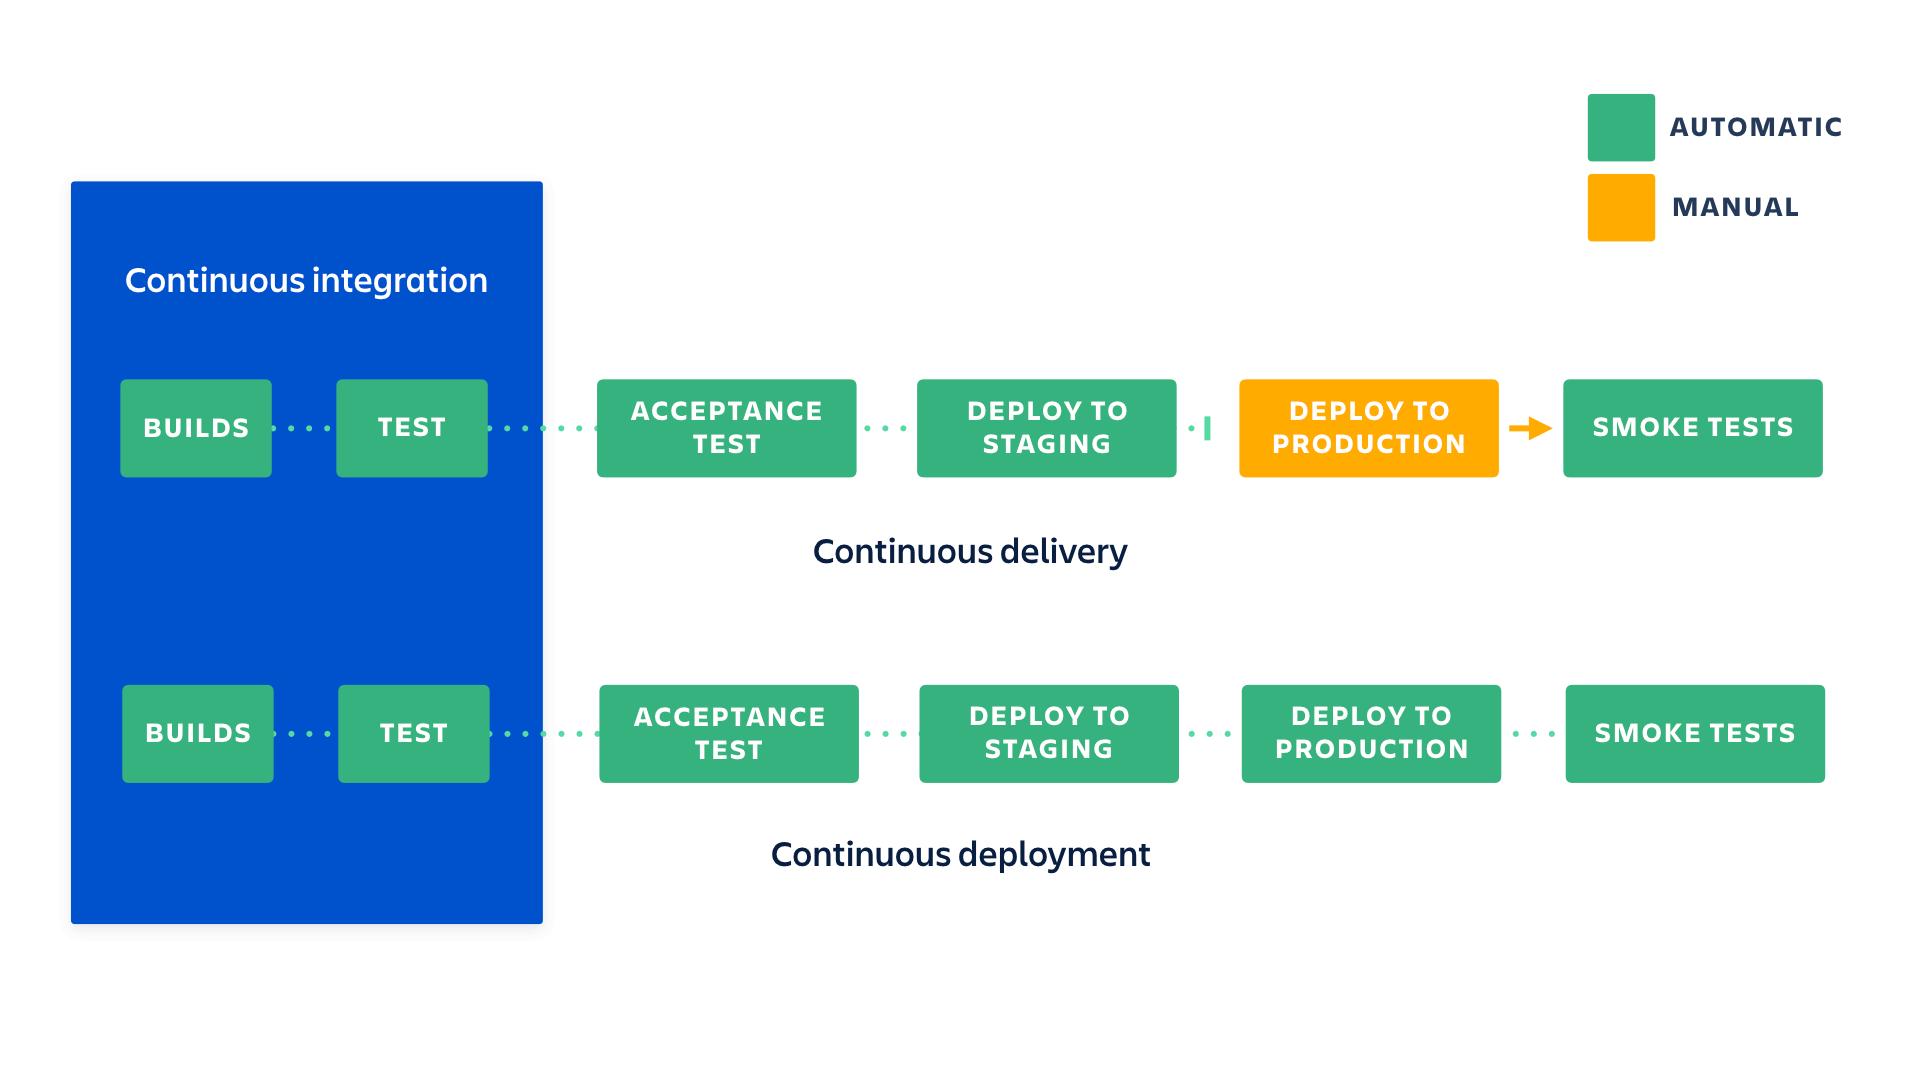
\includegraphics[width=0.95\textwidth]{pics/cicd.png}
    \caption{The relationship between continuous integration, continuous delivery and continuous deployment}
    \label{fig:cicd}
\end{figure}
\subsection{Continuous Integration}
Continuous interaction is the base practice of all practices within CI/CD, and continuous delivery/deployment is based on the continuous interaction.\cite{Continuo67:online}
The continuous integration means the team integrate each team member's work into main codebase frequently(multiple times per day). "Integrate" means merge the code to the main codebase.\cite{fowler2006continuous}. The continuous interaction rely on 2 practices: \textit{Build Automation} and  \textit{Test Automation}. The definition of these 2 practices are:
\begin{itemize}
    \label{TestA}
    \item \textit{Test Automation:} Test automation means using separate software to execute the software automated, without human intervention. It could help the team to test fast and test early. \cite{Testauto48:online}
    \item \textit{Build Automation:} Automate the process of creating software build. This means to automate the dependency configuration, source code compiling, packaging and testing. It is viewed as the first step to continuous integration \cite{Buildaut62:online}
\end{itemize}
With the help of these 2 practices, for each developer in the team, the workflow in continuous interaction as follows:\cite{fowler2006continuous} In the development of each feature, the developer first pull the code from the main codebase. During the development, new test cases could also be added to the automated test. After the development is done, automated testing also runs on the code to maintain the code quality and minimize the number of bugs from the beginning. The build automation compiled the code locally in the development machine. 
\par
After the step above, the developer already has the executable and the high quality (passed the automated test) code in the development machine before submitting the change to the code base. This represents the principle of quality and automation in agile software development. In the next step, the developer commits changes to the repository, which is the main codebase, and the system check the conflict and do the test/build again, to make sure that there are not any bugs missed in the test on the development machine.
If the code passes this build and test, it will be merged to the main codebase and the integration is done.
\subsection{Continuous Delivery and Continuous Deployment}
\label{CD}
Continuous delivery is practices that software development team build a software that can be released at any time of the lifecycle.\cite{fowler2013continuous}This means the software always maintains a high quality and in a deployable state.\cite{WhatisCo47:online} It is a subset of agile, which focuses on the software delivery.\cite{Continuo97:online} From the last section, we introduce the concept of continuous interaction. The continuous delivery is based on continuous interaction but further automate the software deployment pipeline. In the software deployment pipeline, the team divide build into several stages, first build the product and then push the product into the production-like environment for further testing. This ensures that the software could be pushed to production at any time. However, in continuous delivery, the deployment of software into production is done manually.
The benefit of continuous delivery includes:\cite{WhatisCo47:online}\cite{fowler2013continuous}
\begin{itemize}
    \item High code quality: The automate and continuous testing ensure the quality of the software.
    \item Low risk: The software could be related at any time, and it's easier to release and harder to make the mistake
    \item Short time before going to the market: The iteration of software development is much shorter. The automation in testing, deployment, environment confirmation included in the process, and the always read-to-deploy status shorten the time from development to market.
\end{itemize}
The continuous deployment is based on continuous delivery. The only difference is continuous deployment automates the deployment process. In continuous delivery, the software is deployable but not deploy without manual approval. In the continuous deployment, each change that passed automated build and testing will be deployed directly. The continuous deployment is a relatively new concept that most company not yet put the practice into production.\cite{leppanen2015highways} While continuous delivery is the required practice for the company to be DevOps and it is already being widely used.
% \section{Infrastructure as Code}
% The infrastructure is the software infrastructure and configuration needed for the software.
% Infrastructure as code (in short IasC) as it says on its name. is to define the infrastructure with code, and using the tools in the software development to manages these codes which includes version control. \cite{artac2017devops}

\section{DevOps}
\begin{quotation}
    The fundamental goal of DevOps is to minimize the service overhead so that it can respond to change with minimal effort and deliver the maximum amount of value during its lifetime.
    \begin{flushright}
        -- Markus Suonto, Senior DevOps Consultant, Eficode
    \end{flushright}
\end{quotation}
\subsection{Definition}
DevOps is a set of practices that aims to combine different, traditionally separated disciplines (eg. software development, operations, QA, and others) in cross-functional teams with the help of automation of work to speed up software delivery without risking high-quality.\cite{bass2015devops}
\par
DevOps is the extension and evolution\cite{lwakatare2016relationship}\cite{leite2019survey} of Agile. DevOps and Agile both driven by the collaboration ideology and the adoption of DevOps needs Agile as the key factor.\cite{lwakatare2016relationship} DevOps has a different focus on agile. DevOps focus on the delivery while agile is focused on the development with the requirement and customer. Figure \ref{fig:DevOps}\cite{DevOpsin72:online} shows the workflow and practices of a team working under DevOps.
\begin{figure}[h]
    \centering
    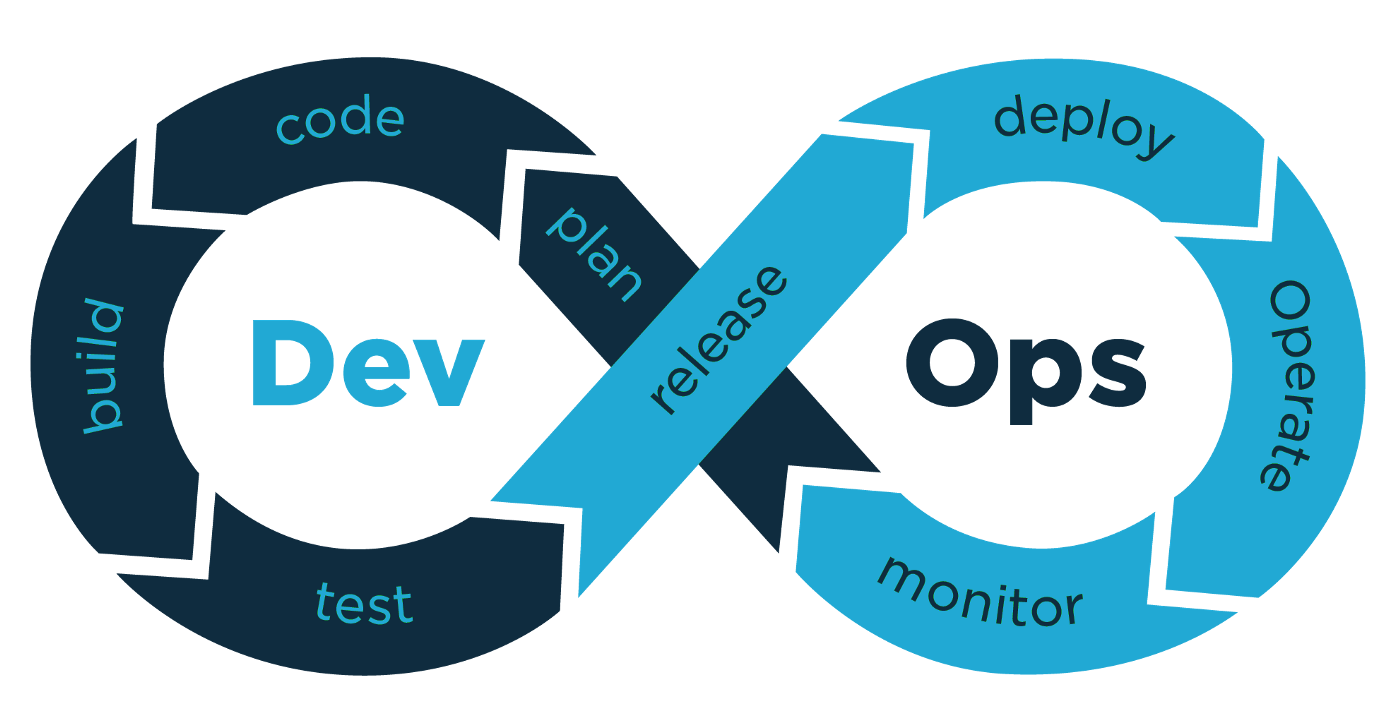
\includegraphics[width=0.95\textwidth]{pics/DevOps.png}
    \caption{DevOps Practices and Workflow}
    \label{fig:DevOps}
\end{figure}
\subsection{Elements}
In this section, we will introduce the necessary elements that an organization need to includes when employing DevOps. 4 necessary elements need to be considered.
\subsubsection[]{Culture}
In the pre-DevOps era, the Development and Operation are two different teams with a different goal.  The interface between them is based on the ticket system which the operation team do the ticket management. As we mentioned at \ref{agile}, the goal of Agile is to shorten the deliver life cycle and delivery software quickly to the costumers. So when practice agile development method under this scenario, the development try to deliver the code they develop earlier but the operation team usually will delay the process for quality control or other reasons. In practice, this causes the delay between the code change and the software delivery to the costumers\cite{leite2019survey}. 
The lack of communication and conflict between developers and the operation team slow down the software delivery process and also make it harder for the teams to be real Agile. Therefore the concept "DevOps" is being proposed at 2008, for eliminating of the boundary between developers (Dev) and operation team (Ops). According to Walls (2013), this is being done by promoting the culture with 4 characterises: open communication, incentive and responsibility alignment, respect and trust.\cite{walls2013building}
\par 
The open communication means openly discussion and debate. As mentioned above, the traditional communication method is through a very formal and regularized ticket system. In the DevOps, the communication is not limited within the formal ticket system. instead, the team will keep in the whole lifecycle of a product, from the requirement, schedule, and anything else. \cite{walls2013building} The information sharing is also important.\cite{lwakatare2015dimensions} The metrics and the project status is available for everyone in the team \label{moniter}, so each member could have a clear scope about what the team is doing.
\par
The incentive and responsibility alignment mean the whole teams (combines Dev and Ops) shares the same goals and also takes the same responsibility. The shift from "Dev" and "Ops" to DevOps requires people who used charges in only development and operation starting sharing the responsibility from both side.\cite{lwakatare2015dimensions} This means individuals or a certain part of the team will be not solely blamed if the product is failed. This "no blame" culture could help each engineer be willing to take the development responsibility for the whole system.\cite{feitelson2013development}
\par 
Respect means all employees should respect and recognize the contribution of other teams members. A DevOps team is not a single team without any division of jobs, there is still an operation part within a team. \cite{TheresNo86:online} However the people operation team will take development responsibility, and the developers will also put their hands-on operation and management.\cite{shropshire2017uncertainty} To make people with different roles works in a team, trust and respect each other is critically important. 
\subsubsection[]{Organisation}
In the organizational level, the DevOps emphasizes the collaboration between different part of an organization. This is strongly correlated with the "culture" part of this section. Inside a team, each member should be a generalist who could understand all aspect of a project. There will not be a dedicate QA, operation or security team within a team. Instead, these are the job that belongs to everyone\cite{feitelson2013development}\cite{kim2016devops} The organization should provide the team member with opportunities to learn all skill needed for building the whole system. 
\par
The team size should be small. A small team could help to reduce the inter-team communication. The small team means the scope of the project is small. And it also means less bureaucracy in team management. There are four benefits to have a small team:\cite{kim2016devops}
\begin{itemize}
    \item The smaller team allows each team member to easily understand the whole project.
    \item The smaller team could reduce the amount of communication needed. It could also limit the growth rate that the product could have.
    \item The smaller team could decentralize power. In DevOps, each team lead could define the metrics which become the overall criteria of the whole team's performance.\cite{kim2016devops} 
    \item In a smaller team, failure doesn't mean a disaster for the company. This allows the team to fail. Thus each employee could train their headship skill in the team without too much pressure. 
\end{itemize} 
\par
Furthermore, another important organizational aspect for DevOps is to have a loosely-coupled architecture. 
The first benefit of this is the better safety.
In the organisation with a tightly-coupled architecture, small changes could result in large failure.\cite{kim2016devops} 
The second benefit is productive. In a traditional organisation, the result of each team will be merged, tested together and deploy together. This means it is time-costly to configure and manage the test environment requires dependencies. A loose organisation enable each team to finish the development of lifecycle (from planing to deployment) independently. Each team could update their products independently, which gives the team more flexibly to align the product with the change in the customer requirement. This means the update of each team's product won't affect other teams as well.
\subsubsection[]{Automation}
In the DevOps, automation means 
automation within the whole development and operation process. The organisations which employing DevOps aims for a high degree of automation.\cite{erich2017qualitative} 
With automation, people could be free from the repetitive work and reduce human error. It could help build the DevOps culture of collaboration, and it is seen as the cornerstone of the DevOps.\cite{DevOpsCu76:online}
The main practices regarding Automation are the automated testing, continuous delivery and automated operation. Automated testing could be achieved by test automation. We already mentioned the benefit of this at \ref{TestA}.
\par
The continuous delivery pipeline is the core of the DevOps.\cite{gill2018devops} As we discussed at \ref{CD}. The continuous delivery will ultimately automate all steps between the developer to commit the code to the product in the production.
\par
The automation of the operation part is usually done by using the concept of "Infrastructure as Code"\cite{lwakatare2015dimensions}. The Infrastructure as Code (IasC) means to define everything in the software infrastructure level as code.\cite{artac2017devops} Because it is code, we could use the automation methodology used in the software development to manages and deploy these codes. According to Christof et. (2016), under IasC, infrastructure can be shared, tested, and version controlled. \cite{ebert2016devops} This could help emphasizes the automation within the operation scope. With the automation in operation, the team could be free from the tedious environment configuration and shorten the product development lifecycle. Automating server configuration means the developers and operation staff can equally know the server configuration \cite{DevOpsCu76:online} which help build the culture of shared responsibility and trust.
\subsubsection[]{Monitoring}
Monitoring is to continuously collect the matrices from the running system for helping the team find the problems in the system.
In the DevOps way of development, the testing is the key to maintain the quality of the software continuously. However, when the product enters the production, we cannot test the software any more. So, we need monitoring to keep track the status of the product.\cite{huttermann2012devops} Thus, Monitoring is an important component of DevOps.
\par
With monitoring, the software team could keep tracking the status, and maintain the quality of deployed production. The monitoring has also enabled the team to collect the data from costumers' usage behaviour. This helps the agile development team to make an improvement in the next iteration of the product. \cite{lwakatare2015dimensions}
\par
For develop a high-quality monitoring system, the development of monitoring could be in parallel with the main product, and the monitoring system can be already be used against the "staging deployment" (see Figure \ref{fig:cicd}) at the early stage of the iteration. By this, the development team can improve the monitoring system continuously together with the main software system. The parallel development of the monitoring system and the main system helps the team to find the gap in the monitoring earlier.\cite{huttermann2012devops}
\par
On the other hand, As we mentioned in the "Culture" section, the collaboration is an important part of the DevOps culture. collaboration needs the communication and information sharing between the development(Dev) and operation(Ops) team. The monitoring could be one of the channels between the Dev and Ops since it can expose the information of the whole system which helps team members to understand the system as a whole. This helps the team achieving the point we mentioned at \ref{moniter} (Culture) that the project status and matrices should available to every team members.
\subsection{DevOps Practices}

\chapter{Literature Analysis of the Cloud Technologies}
In this Chapter, we will do an literature review on the new cloud technologies which emerged in recent years. 
\chapter{Design of DevOps Toolchains}
In this chapter, we will introduce the design and implementation of DevOps toolchains.
Note that for the experiment that is answering RQs in Chapter 5, we implement two different continuous delivery pipelines design with two sets of tools respectively, one with tradition non-integrated tool while another one with the serverless integrated DevOps tools from AWS. In conclusion, we introduce the design of both toolchains(server-based and serverless) and explain how we come to this implementation in this chapter.
We will also compare these two types of toolchains within the scope of functionality and ease of implementation.
\par
In Section 4.1, we present the case software project developed by us that will be built, tested, and deployed by our DevOps toolchain in the experiment. In section 4.2, we introduce the design and implementation of our non-integrated DevOps toolchain. Section 4.3 is related to the integrated toolchain.
\section{Case Project}
We first develop the case project. The case project is an example software project which will be used to test our implementation and run the experiments. This means we will simulate the DevOps development process of the case project on our DevOps toolchain. Although the type of our case project has no effect on our DevOps toolchain on the architecture level, the build dependencies and the software configuration inside our toolchain could be affected by it. Thus we must have an introduction to the case project.
\subsection{Programming Language and Framework Considerations}
Java is one of the most common languages used in commercial software development. According to the TIOBE index of programming language \cite{indexTIO42:online}, Java is the most popular or the second most popular programming language in the world since the mid-1990s. Besides commercial software development inside companies, Java programming language is widely used in open-source software development. The report \cite{TheState3:online} from GitHub shows that Java ranked third most popular programming language in 2019, and it ranks second before 2018. Furthermore, Java has good versatility, which means it almost every kind of applications. For instance, web applications, desktop applications, besides, Java is the main development language for Android applications.
\par
To the DevOps point of view, the Java programming language has a complete ecosystem. The complete ecosystem means there are tools for every phase of Java application development. These tools include: build, code analysis, testing frameworks, artifact management, build automation \& dependency management et. These tools could be easily integrated and act as part of the DevOps toolchain.
\par
Therefore, due to the popularity, versatility and complete ecosystem of Java programming language, we select Java as the language of the case project.
\par
One of the major application of Java in web development. Currently, 7 out of 10 \cite{Programm17:online} most popular website is using Java as a web development language (server-side). In the field of web development, Spring framework is the most popular framework for Java, and it is being used in many major internet companies including Google, Microsoft and Amazon \cite{SpringWh14:online}.
\par
So, we choose Spring the framework to build our application. To develop our Spring application, we use Spring Boot\footnote{https://spring.io/projects/spring-boot}. Spring Boot is a project under Spring, which, according to its documentation, is to allow the developer to create Spring application with the minimal effort \cite{SpringBo84:online}, by simplifying the configuration of Spring framework.
\subsection{Project Description}
\begin{figure}[!h]
\begin{verbatim}
Method: GET
Endpoint: /packages
Success Response:
Code: 200
Content:
[
{
name : (Package name)
description : (Package description)
dependencies : (Dependencies)
}
]
Error Response:
Code: 500
Content: { msg: Server Error! }
\end{verbatim}
\label{fig:rest}
\caption{RESTful API Interface of Case Project}
\end{figure}
The case project is a simple REST API (Figure \ref{fig:rest}) which returns the info of all installed software packages in the host machine in JSON format when the frontend sends an HTTP GET request to the backend.
\section{Design of Non-integrated DevOps Toolchain}
In section, we present our design of DevOps toolchain, which is non-integrated. Part of the components is still based on the virtual machine. Each section is the introduction to the design of each component. We also present the consideration when a select tool for this part of the toolchain in each section. Besides, in each section, we introduce how could serverless computing be used by this component in general and the benefits to the specific tool we select.
\subsection{Architecture}
\begin{figure}[!htbp]
\centering
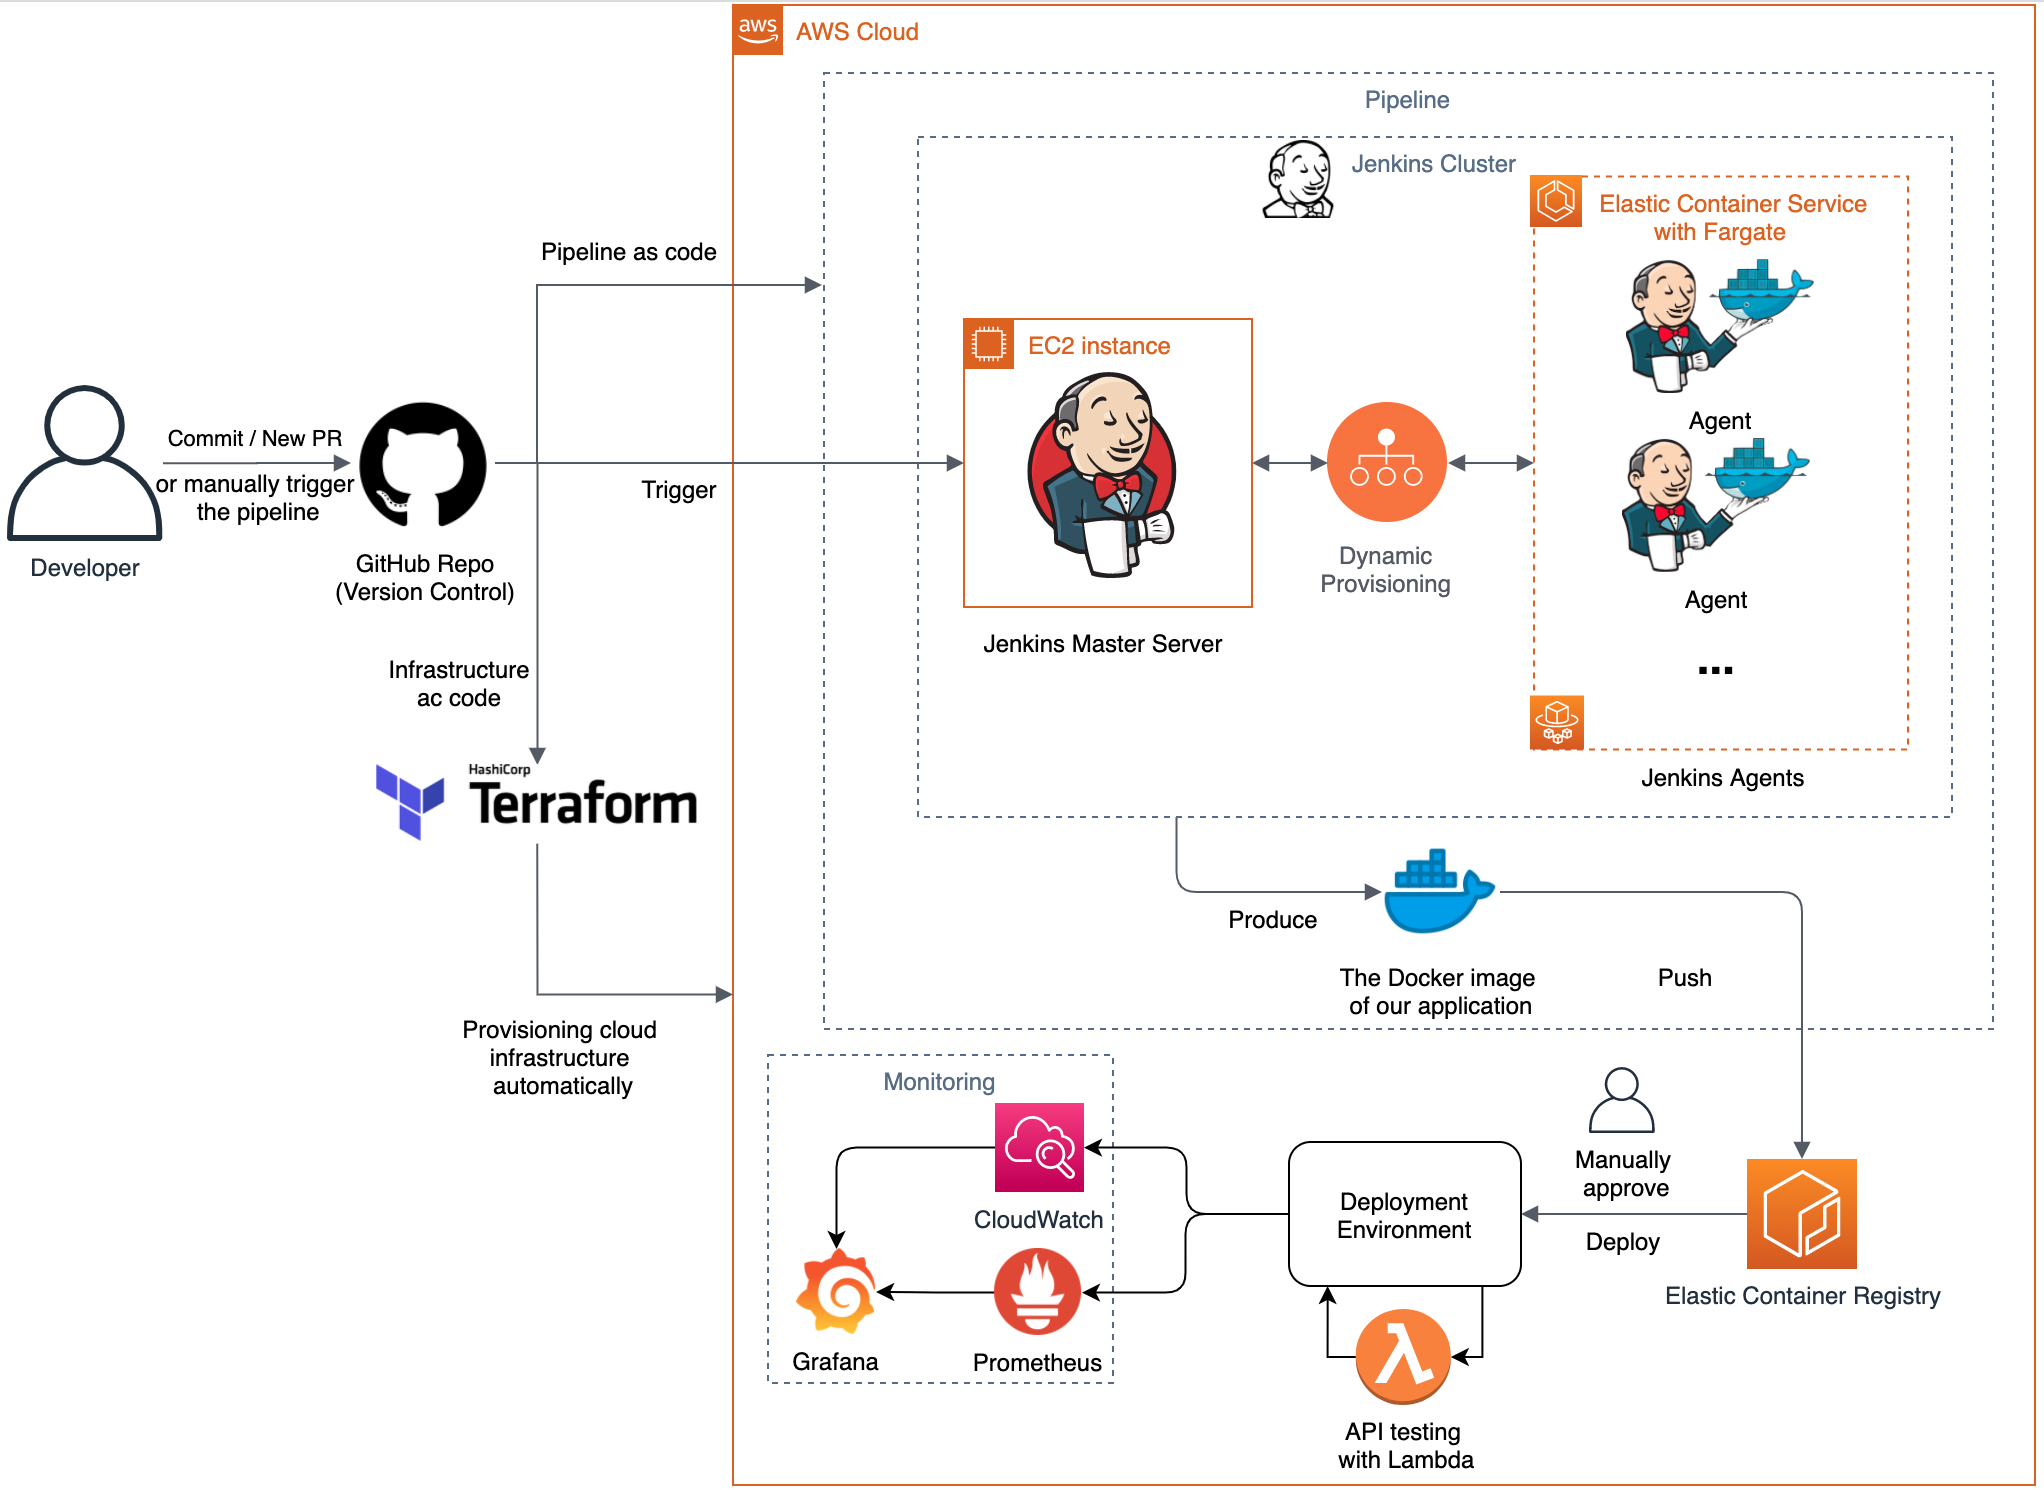
\includegraphics[width=0.99\textwidth]{pics/arch-med-jenkins.png}
\caption{Architecture diagram of our DevOps toolchain}
\label{fig:archjenkins}
\end{figure}
The toolchain implementation is based on the DevOps elements we presented in Chapter 2, and the DevOps practises from Eficode. Figure \ref{fig:archjenkins} shows the architecture of our DevOps toolchain. In here we are only presenting architecture on a more general level. The detailed architecture of each component will be introduced in the following sections, both text and graph.
\par
When the developer pushes a new commit to the repository in GitHub \footnote{https://github.com/}, Github will send an HTTP POST request that contains the necessary information to the Jenkins master node. Jenkins master, which triggered by the HTTP request, will create a new job for this project according to the information that the HTTP request contains. The job will first pull the latest code from the git repository, then runs the docker containers with required build environment and build the project. In the end, a docker image for running the project will be created and be pushed to the container registry of AWS. Depends on the git branch that the developer committed to, the project will be deployed to a different development environment.
\par
Figure \ref{fig:archjenkins} shows the architecture of our DevOps toolchain. We can see except version control, and the whole environment is running in Amazon Web Services. Due to the limitation of space, the internal architecture of certain components is not shown in the graph. Instead, we show them in the following sections.
\subsection{Tool Selection Considerations}
One of the essential steps to build the non-integrated toolchain is to select the proper tool for each component.
In this section, we describe our consideration when we select tools.
\paragraph[]{Continuous Delivery Pipeline}
The most popular server-based tools for build continuous delivery pipeline are Jenkins\footnote{https://www.jenkins.io/}, Drone\footnote{https://drone.io/}, GoCD\footnote{https://www.gocd.org/} and Circle CI\footnote{https://circleci.com/}. A comparison between these tools is shown in Table \ref{tab:ci-tools}. As we can see from the table, Jenkins is the most popular option for CI/CD. Jenkins has wide application in the commercial use case, and the high popularity in the open-source community as well. Although compared with the other three newer tools, Jenkins is more focuses on the "Build" step within the continuous delivery pipeline. Nevertheless, the open-source nature of Jenkins gives it a much wider selection of the plugin, which means Jenkins can be used for almost all steps in a continuous delivery pipeline.
\begin{table}[h]
\begin{tabular}{|l|l|l|l|l|}
\hline
& Jenkins & Drone & Circle CI & GoCD \\ \hline
Open Source & Yes & Yes & No & Yes \\ \hline
GitHub stars & 15.7k & 21.2k & - & 5.7k \\ \hline
Github contributors & 614 & 258 & - & 116 \\ \hline
Plugin extensions &
Over 1500 \tablefootnote{https://plugins.jenkins.io/} &
93 \tablefootnote{According to GitHub search result} &
110 \tablefootnote{https://circleci.com/integrations/} &
88 \tablefootnote{https://www.gocd.org/plugins/} \\ \hline
\begin{tabular}[c]{@{}l@{}}Price of self-hosted \\ solution\end{tabular} &
Free &
Free &
\$35 user/month &
Free \\ \hline
\begin{tabular}[c]{@{}l@{}}Number of companies\\use it in the tech stack\tablefootnote{based on data from StackShare}\end{tabular} &
2634 &
82 &
1368 &
42 \\ \hline
\end{tabular}
\caption{Comparison of continuous delivery tools}
\label{tab:ci-tools}
\end{table}
\par
Created by Kohsuke Kawaguchi in 2001, Jenkins is an open-source continuous integrating tool write with Java. It is suitable for a team of all sizes and varies of languages and technologies \cite{smart2011jenkins}. Furthermore, Jenkins also attracts software teams with its easy-to-use and high extendibility \cite{smart2011jenkins} with a thousand of the plugin. More plugin keeps coming since Jenkins has an active open-source community. These plugins help Jenkins keep up with the fast-developing DevOps practices, and help Jenkins integrate with the newly emerging tools and cloud services. The extendibility makes Jenkins still the most popular tool for DevOps toolchain even it is an aged software created when the term "DevOps" just appeared.
\par
Our continuous delivery pipeline is built with Pipeline plugin\footnote{https://www.jenkins.io/doc/book/pipeline/} in Jenkins.
Pipeline plugin allows us to define a continuous delivery pipeline as code in Jenkinsfile.
In the pipeline, a conceptually distinct subset of tasks within the continuous delivery pipeline \cite{Pipeline85:online} is defined as a "stage"\footnote{For example, "Build", Test", "Deploy" step in a continuous delivery pipeline.} and each task within a step is called "step". Each pipeline is binding with a "project". An execution runtime of a project/pipeline is called "build", and the machine (virtual machine, container, e.t.) for running the build is called "agent".
\paragraph[]{Build \& Test Automation Tool}
For the build stage within Jenkins pipeline, we use Gradle\footnote{https://gradle.org/} as the build tool.
Gradle is a powerful build tool initially designed for JVM based language, but now it also supports other programming languages, for example, C++ and Python. Like Jenkins, Gradle also has a dynamic ecosystem with thousands of plugin. This enables the possibility to use different kinds of tools such as unit testing and code analysis within a single pipeline of Gradle. Gradle also makes the dependency management easy, and dependencies could be easily added to the project by editing the Gradle configure file of the project. Furthermore, Gradle supports configuration as code. This allows developers to define all the build configurations of a software project in a single file.
\par
For unit testing within the build stage, we are using JUnit \footnote{https://junit.org/junit5/} as the tool for testing. For code analysis, we use SonarQube\footnote{https://www.sonarqube.org/}. Both are one of the most common used tools in their specialized field in the Java ecosystem. Moreover, both tools have official Gradle plugin, which allows us easily use them with Gradle.
\paragraph[]{Deployment and Jenkins Agents}
We will widely use Docker \footnote{https://www.docker.com/} in our pipeline.
Docker is an open-source software which could pack, deliver and run the software as a container. A container is a separate unit that includes the application and all its dependencies which allow application runs in the same way regardless of the host environment \cite{WhatisaC60:online}. A container is the running instance of a Docker image that defined by Dockerfile.
\par
\label{docker}
There will be two main use cases of Docker in our toolchain. Firstly, we run the build stage within the container.
Nowadays, Docker\footnote{https://www.docker.com/} is being widely used as build agents in continuous integration and continuous delivery (CI/CD) pipelines.
This means the pipeline will execute specific steps inside ephemeral Docker containers \cite{Overview44:online}. It is easier to manage build dependencies in the Docker container. Besides, the container-based agent requires less effort to maintain.
\par
In our case, to build the case application, the host machine needs to have JVM installed. However, we want to make our pipeline not only suitable for Java application but also easily be used to build an application in other programming languages. Docker solves this problem by provides excellent isolation from the host machine. Thus, we can configure the built environment (operating system version, dependencies) runs within a Docker container without actually install anything on the host machine by merely editing the Dockerfile.
\par
We also use Docker to Dockerize our application which creates a Docker image of our application.
Docker allows us to specify all system dependencies in a single file (Dockerfile), so there is no need to have any Java environment pre-installed in the deployment environment which runs our application. This is because all environment is already being packed in our Docker image. By doing this, firstly, we reduce the operational effort. Secondly, we improve compatibility since Docker makes sure that the docker image could run in the same behaviour no matter what host machine it runs on. Also, all major cloud computing providers support Docker. We could easily run the container from our Docker image on their VM, and they are serverless computing services. This means our Dockerized application could easily be cloud-native and be deployed across a multi-cloud environment.
\subsection{Infrastructure as Code (IasC)}
Configuration Management is one of the component of DevOps toolchain that we mentioned in Chapter 2. Infrastructure as code the common practices to implement configuration Management in the cloud-based environment.
\begin{figure}[h]
\centering
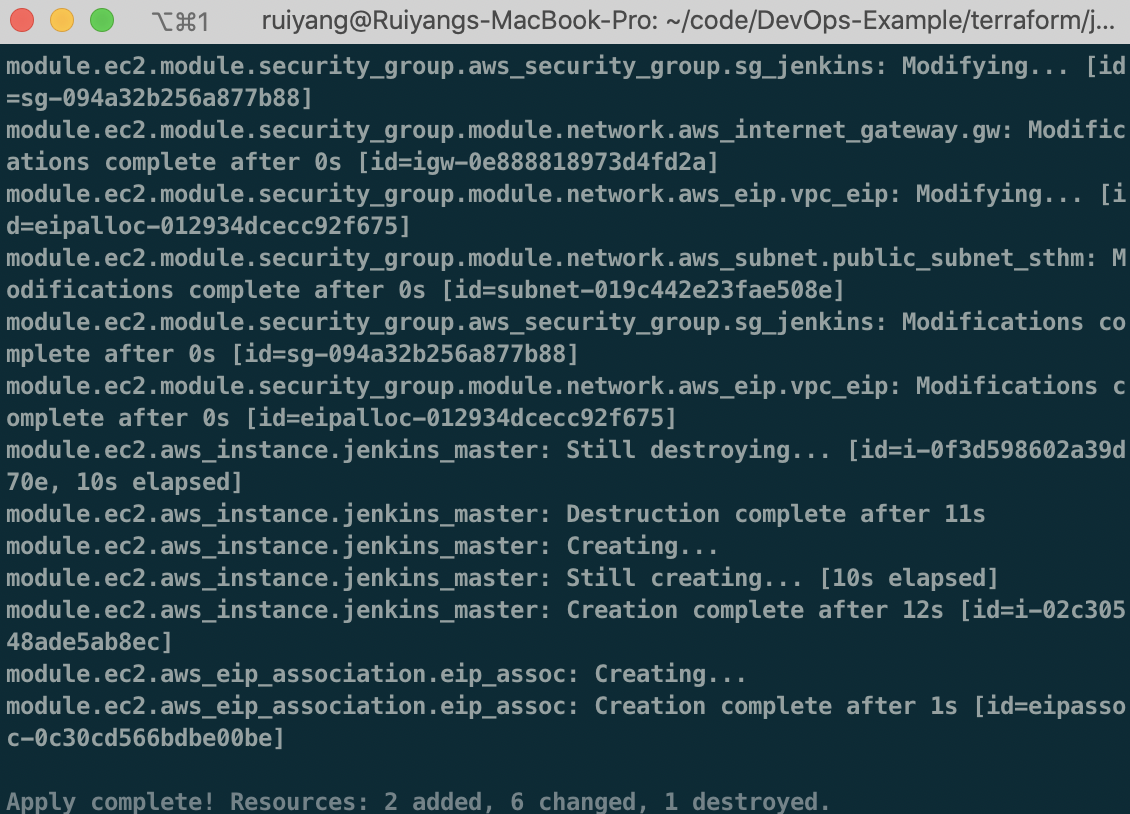
\includegraphics[width=0.99\textwidth]{pics/terraform.png}
\caption{Creating a cloud environment with Terraform CLI}
\label{fig:terraform}
\end{figure}
\par
Terraform \footnote{https://www.terraform.io/} is one of the most popular tools to manage cloud Infrastructure with IasC practice. It has the thorough support of AWS. In our implementation, we define our could infrastructure and all AWS resources including EC2 virtual machine, ECS cluster, security groups and network Infrastructures in a series of configuration files. Then we create the cloud environment by simply using CLI interfaces. Figure \ref{fig:terraform} shows the creation of the cloud environment with Terraform.
\subsection{Version Control}
Version Control System (VCS) is the process that record the changes in files set over time \cite{GitAbout93:online}, and versioning the history of these files. VSC is suitable for track the development progress and manages the goal within a software development team \cite{loeliger2012version}. Among all software for version control, Git is the most popular one nowadays. The survey \cite{CompareR31:online} from Synopsys shows that in 2019, 71\% of the project today is using Git as it is versioning system while SVN that ranks in second only be used in 25\% of the projects. We use Git as the version control system since it is used by most of the software development teams nowadays. We use GitHub for hosting the case project. Github is the biggest preform in the world that hosting a version-controlled software project for free using Git. It provides interfaces with different DevOps related tools which makes it easy to be integrated into all kinds of DevOps toolchains.
\begin{figure}[h]
\centering
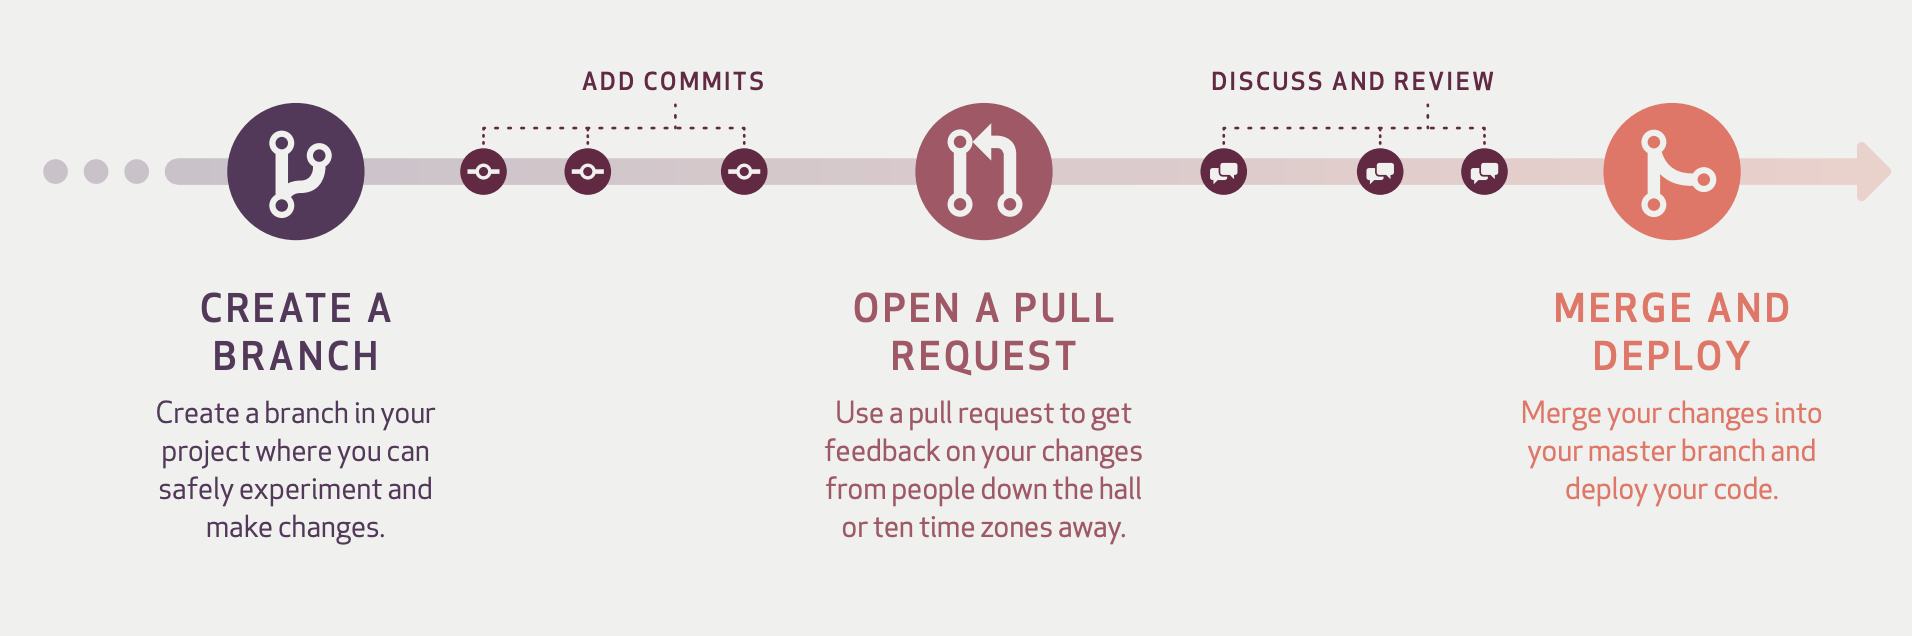
\includegraphics[width=0.99\textwidth]{pics/git.png}
\caption{GitHub Workflow \cite{guides2013understanding}}
\label{fig:git}
\end{figure}
\par
The Git flow \cite{driessen2010successful} proposed in 2010 is a successful workflow for working with Git. Git flow has already widely used and has been approved by the software industries. However, to better cope with the frequent release nature of DevOps, the Github workflow -- a simplified version of Git flow is proposed by GitHub.
Therefore, GitHub workflow \cite{chacongithub} is being chosen as our workflow in the version control. The simplified version of this workflow is shown as in Figure \ref{fig:git}
\par
Several general principles followed by us when adapting GitHub flow, we refer to principals in \cite{chacongithub} to design our workflow.
\begin{itemize}
\item Master branch is always deployable. This means when deploying the continuous delivery pipelines in our toolchain, only the master branch can be deployed. Moreover, there should not have any code which is not good to be deployed in the master branch.
\item When working on the new feature, make a new branch for this feature. The name of this branch should be descriptive, which reflect the content of this feature. Commit the code related to this feature this branch and push from this branch to the branch with the same name on the remote server (github.com).
\item Open a pull request\footnote{https://help.github.com/en/GitHub/collaborating-with-issues-and-pull-requests/about-pull-requests} when the feature is ready to merge, or when developer feel that he/she need help or comments from other team means on this feature. Others also do the code review in the pull request.
\item When the code is already be reviewed and is good to be merged, the developer should merge the code to the master.
\item After the code of this feature is in the master, the code will and should be immediately deployed. There should not be any rollback in the master branch. If there are any issues within the newly merged code, a new commit or a new branch should be made to fix the issue rather than rollback on the master.
\end{itemize}
\par
Note that in our Git workflow, there are several time points that we need to run the continuous delivery pipeline within the toolchain. The continuous delivery pipeline will also vary with the time point within the version control workflow. We will introduce this in detail on \ref{our-ci}.



\subsection{Continuous Delivery Pipeline with Jenkins}
\label{our-ci}
\begin{figure}[h]
 \centering
 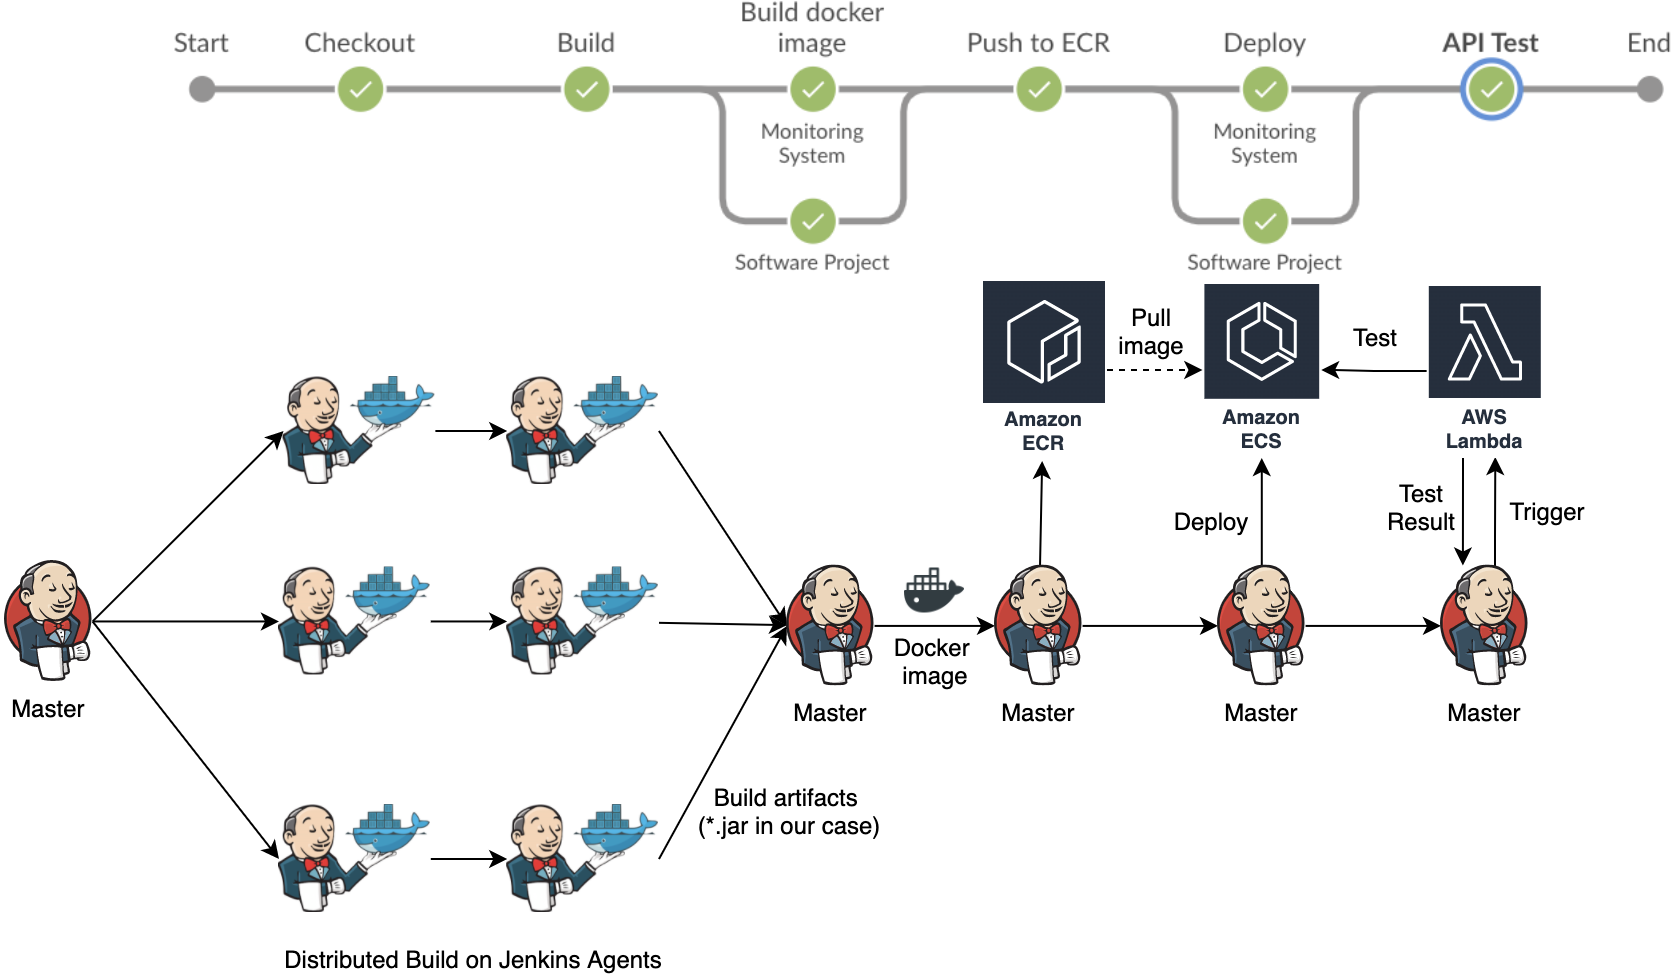
\includegraphics[width=0.95\textwidth]{pics/overview.png}
 \caption{The Stages and Distributed Build in Our Pipeline}
 \label{fig:overview}
\end{figure}
Figure \ref{fig:overview} shows the five stages in our pipeline that shown in the Jenkins dashboard. The bottom part of this Figure shows the task distribution between the master node and agent nodes. The master node is an EC2 virtual machine while agents run on Fargate instances within an ECS cluster.
\par
As we can see from the Figure, when the master node starts a job, it will create a Docker container in AWS Fargate as the agent. The agent will pull codes from VCS, build the code, and then send the build artifacts back to the master node. After this, the container will be terminated. The master node will continue the rest steps.
\paragraph[]{Build Agents}
Build agent is an independent computation unit (VM or Docker container) that could exchange data with the Jenkins master node and run a certain part of the pipeline. To implement a Jenkins build cluster, we need first to implement build agents.
We discussed why we use Docker-based agent in our Jenkins build a cluster on \ref{docker} and we decide to it in our implementation. The first step of our implementation is to develop our own Docker image \footnote{The Docker image we developed could be found at https://hub.docker.com/r/dry1995/jnlp} of the Jenkins agent. We use the "jenkins/jnlp-slave"\footnote{https://hub.docker.com/r/jenkins/jnlp-slave/} as the base image, this allows our Jenkins agent to establish an inbound connection to the Jenkins master with TCP. The next step is to set up the built environment within the agent. We add shell script for auto-install all build dependencies to build our case project when we build this Docker image. In the last step, we build the Docker image for build agent and push it to DockerHub. 
\par
We also discussed how Fargate allows us to run container serverless. To make use of Serverless offering of AWS, we let Docker-based Jenkins agents run on AWS Fargate to cut the operational effort and automate the scaling of Jenkins cluster. To implement this, we use Jenkins plugin "Amazon Elastic Container Service (ECS) / Fargate, which is the only Jenkins plugin allow us to host Jenkins agent in Fargate.  
\paragraph[]{Considerations in Designing the Workflow of Distributed Pipeline}
The considerations behind to our design are that the first two steps take most of the time in our pipeline and according to Figure \ref{fig:pipeline} runs more frequently than other steps \footnote{The reason will be discussed in next section "Workflow in Production"}. The running time will be further extended when building a larger project. These two stages will be the bottleneck of the pipeline if we have it on the master mode. So we need to offload these steps to Jenkins agents for better performance.
\par
The second reason is: as we mentioned in our introduction of Docker at \ref{docker}, the built environment inside Jenkins agents that runs in Docker container is easier to be changed. When the team want to build the same code for different OS (Which happens in C/C++ development) or want to have a different build environment for different projects, they eliminate tasks such as configuration and installation different environment thanks to Docker. Instead, they can just modify the Dockerfile that defines the Docker image of the Jenkins agents. However, we cannot put the stage that builds a Docker image in Jenkins agents. This is because AWS Fargate does not allow building agent runs in a free container which means we cannot use Docker within the Jenkins agent's container that runs in Fargate. This is one significant limitation of Fargate, so we have to move the step back to the master node. Fortunately, in our case project, the Docker build only takes a short time (<1s on average). Therefore this will not slow down the whole pipeline.
\par
We also notice that the Deploy stage also takes a long time. Still, we do not have it in the distributed build because: first, it is on the end of a pipeline so it will not block the further steps, second, the pipeline runs the stage less frequently than first two stages as shown in Figure \ref{fig:pipeline}. Thus there will be less possibility that there are many jobs runs at "Deploy" stage in parallel.
\begin{figure}[h]
 \centering
 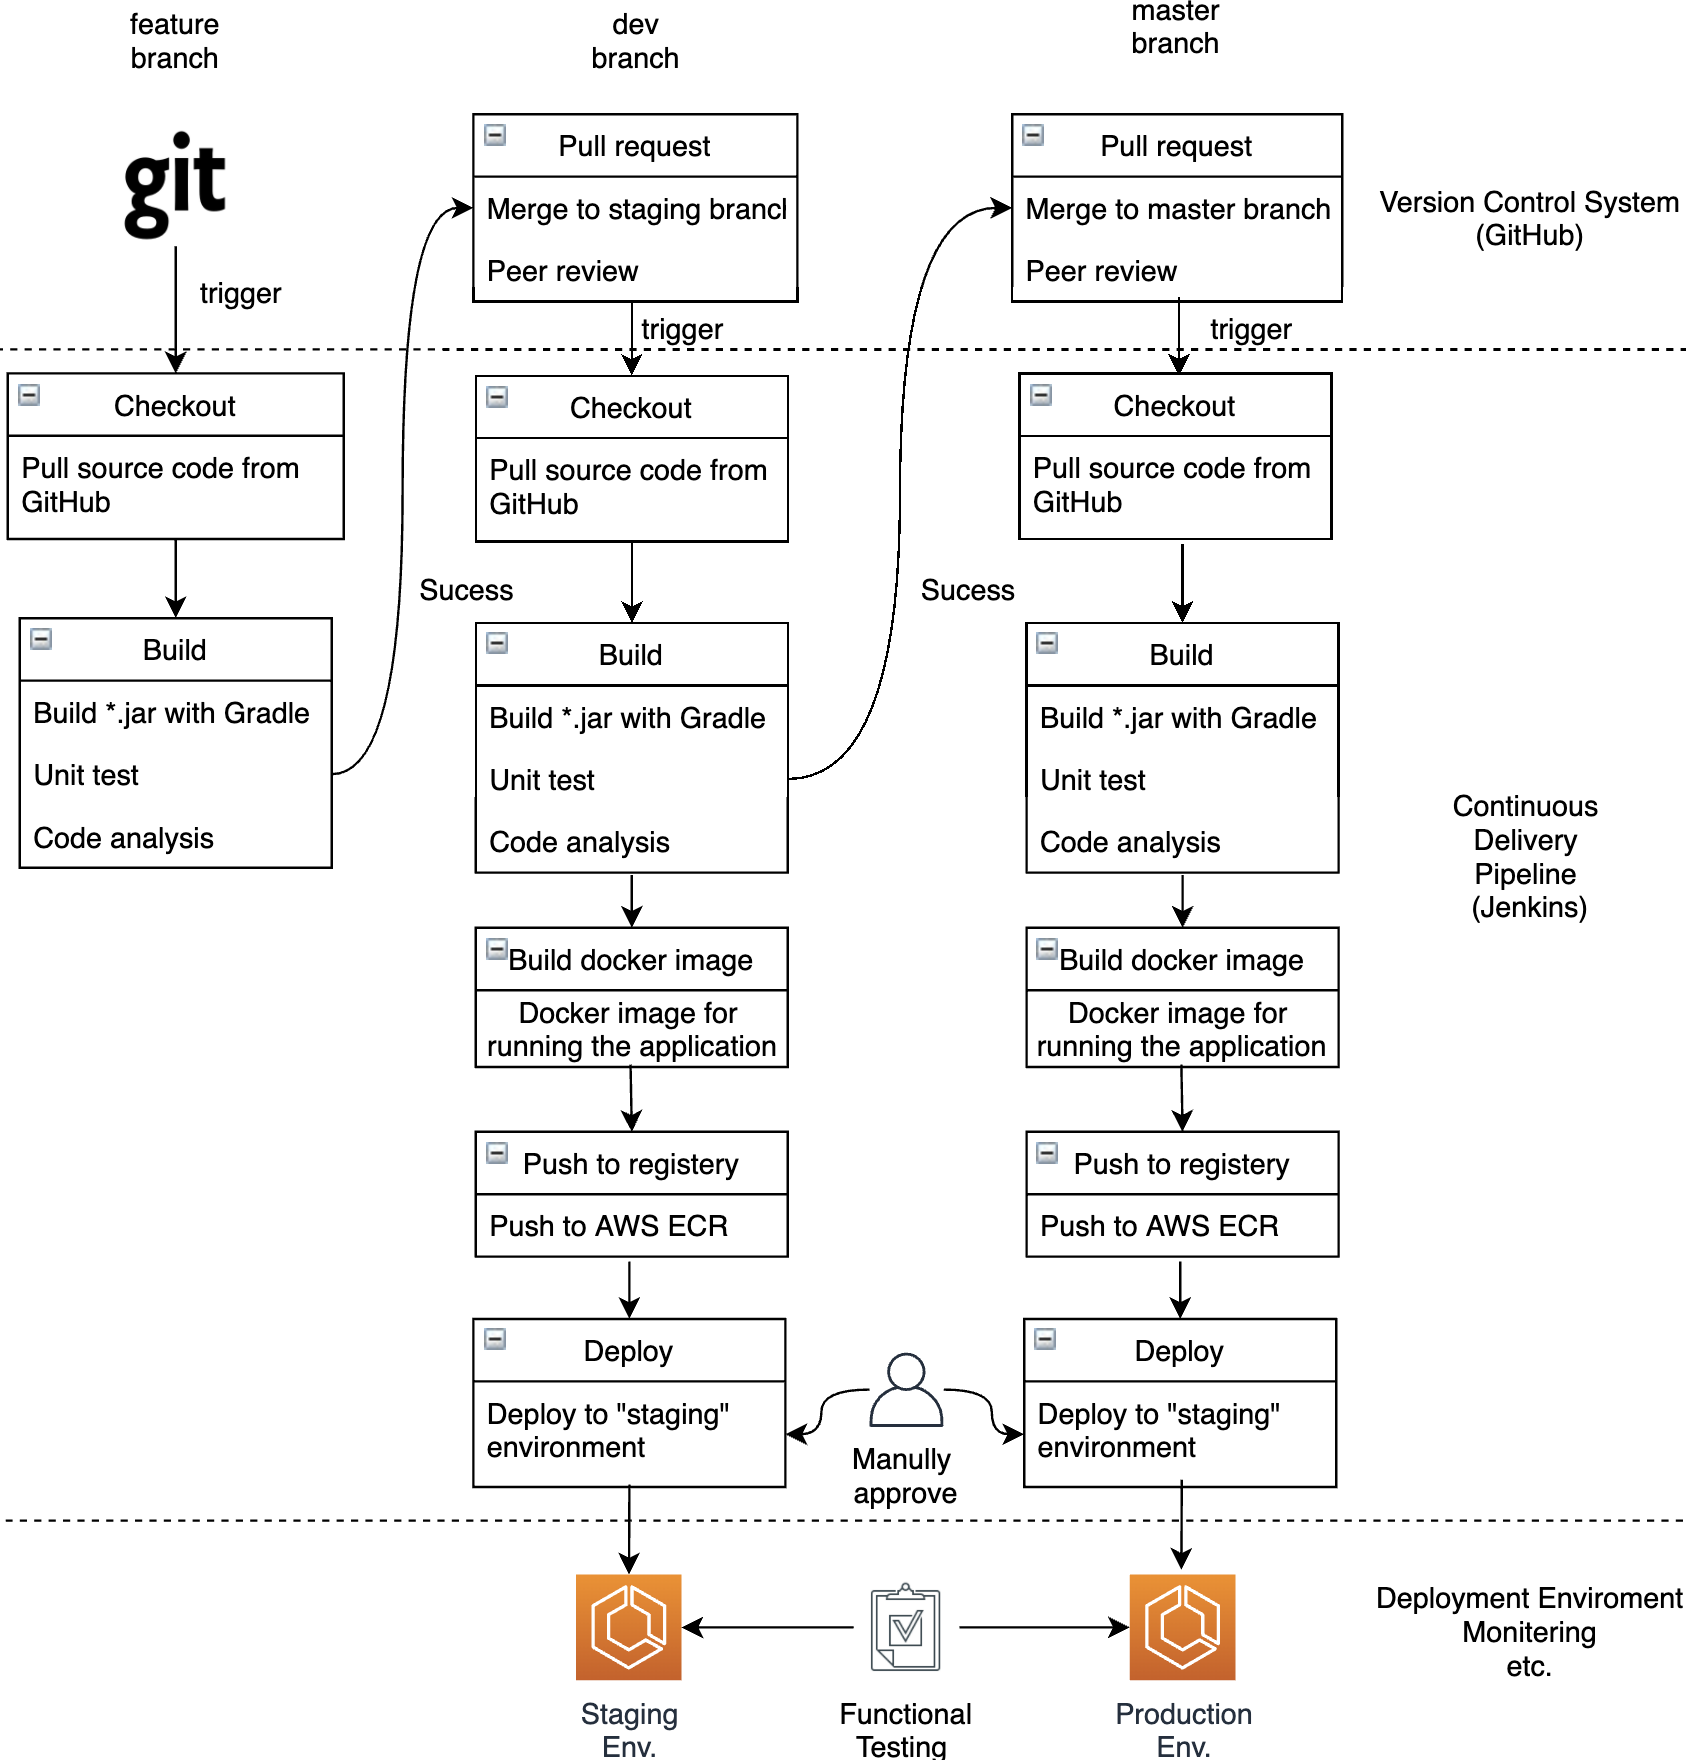
\includegraphics[width=0.99\textwidth]{pics/pipeline.png}
 \caption{The Workflow of Continuous Delivery Pipeline in Our DevOps Toolchain}
 \label{fig:pipeline}
\end{figure}
\paragraph[]{Workflow for Continuous Delivery}
Figure \ref{fig:pipeline} shows the workflow of a project that goes through our continuous delivery pipeline.
We can see when the event on the feature branch triggers the pipeline, and it only runs through the first two stages. This is because according to the practices of continuous integration mentioned by us in \ref{CD} and by Martin Fowler in \cite{fowler2006continuous}, a developer should merge(the "integration" in continuous integration) his/her work couple times per day. Therefore the whole pipeline will run the code with this new feature at least several times a day. This already ensures the code could frequently be tested and deployed into the test environment. Thus, in the pipeline runs after the push to the feature branch, the further steps could be skipped. 
\par
 The developer only commits to the feature branch. The pipeline runs first two stages after a developer pushes local commits to Git. It first pulls the newly pushed code, and then build. In the build stage, the code first is analyzed, then we do unit testing to make sure the code could pass the test cases defined by the developer during development. In the end, the code will be built into Java ARchive file (.jar). The purpose of putting code analysis step first is that the code analysis will check syntax error and bugs. We want to make sure the code is runnable, and no syntax error before put it into the build. So we can reduce the cost by reducing pipeline running time if there is error exists in the code. 
\par
If no error returns after finishing all the above steps, the developer can open a pull request view the code change and ready to merge the code to the dev branch. Before the merge, the pull request needs to pass the code review by another developer. Code review is to make sure that the automated tests do not miss any bugs. After the code review passed, the reviewer or the developer him/herself merge the code to the dev branch.  
\par
After the code merged to the dev branch, the pipelines run again, this time it runs the whole pipeline. First, the pipeline executes the first two stages as in the feature branch. Now we have the Java ARchive file. The Java ARchive is an executable package of our Spring Boot application. Next step is to Dockerizing our application which generates the Docker image our application. Then we push the image to the Amazon Elastic Container Registry AWS (AWS ECR) for further use.
\par
\label{deploy}
The last step of the pipeline is deployment, the pipeline pull image in ECR that we pushed in the last stage, and then deploy it to the deployment environment in ECS with AWS CIL. The deployment strategy we are using is the rolling update. In the rolling update, we are gradually replacing instances in our deployment environment with the newer version of code.
\par
In the dev branch, we deploy the application to the staging environment. The deployment to staging environment should be automated. This is because the staging environment is only for testing and only visible within the team. 
In the staging environment, we will conduct functional testing for test if our deployed API works and if it works as expected. If the deployed function passes the smoke test, this shows the deployment works as expected and ready for the deployment. The developer could now open a pull request, merge code to master branch. The pipeline will runs again, and deploy the application to the production environment, which is visible to the costumers.

\subsection{Deployment Environment}
\begin{figure}[h]
 \centering
 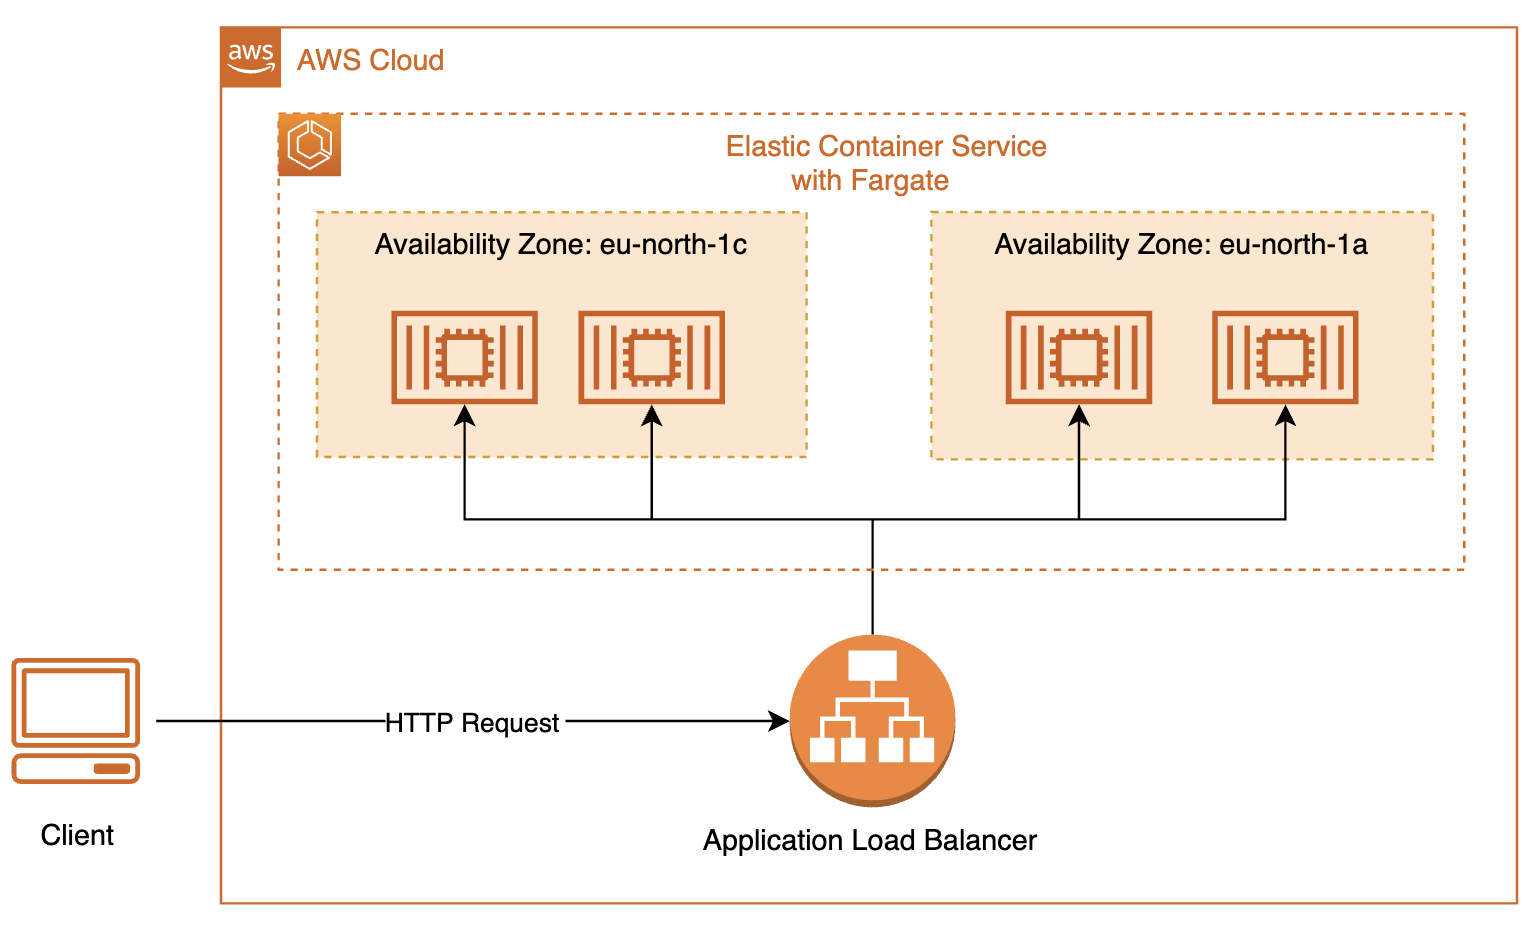
\includegraphics[width=0.99\textwidth]{pics/deploy.png}
 \caption{Deployment Environment}
 \label{fig:deploy}
\end{figure}
We create a simple deployment environment with AWS Elastic Container Service and Elastic Load Balancer. Same with Jenkins agents, we use Fargate to host our containerized case project. 
\par
AWS Fargate allow us to run our containerized application without having to manage servers, makes it easier for us to build a functionality complete DevOps toolchain implementation. We choose ECS over EKS (Elastic Kubernetes Service) is because ECS is free of charge while EKS charges extra for the runtime of the cluster. Compared with EKS, ECS also provides better integration with other AWS services, such as with AWS DevOps toolchain, and AWS CloudWatch monitoring.
\par
Figure \ref{fig:deploy}
shows our deployment architecture. The deployment region in Stockholm(EU-north-1). The Fargate instances in ECS cluster are automated scaled according to the number of incoming requests. 
To improve the availably of the product, we deploy the case project into two different availability zones within the region. 
When one availability zone is down, the load balancer can route the request makes sure the request can still reach the healthy availability zone. Besides the availability improvement, the load balancer also distributes incoming requests across Fargate instances which maximizing the resources rate within our ECS cluster.
% During deployment, we use Martin Fowler's blue and green deployment strategy \cite{fowler2010bluegreendeployment}, which is natively supported by ECS. This means when a new deployment comes, the older version will continue serving until the newer version reaches the stable status. This could significantly reduce the downtime in the deployment. 
% \subsection{Smoke Testing}
% Testing is an implement component within the DevOps pipeline
% In this section, we further discuss the smoke testing that we mentioned in the \ref{deploy}.
\subsection{Monitoring the Deployment}
Monitoring is one of the important components in the DevOps toolchain. Different from testing, which usually integrated with the continuous delivery pipeline, the monitoring is independent of the pipeline. Usually, monitoring does not act as one step within the continuous delivery pipeline but as an independent component.
\par
In Chapter 3, we introduced AWS CloudWatch as one of the serverless services in AWS. In our toolchain, we will use it as the primary tool for monitoring. With Cloudwatch, we not only can get the realtime log from our deployed container in the ECS but also the quantitative data, for example, memory utilization and network i/o, the monitoring dashboard can seem at figure \ref{fig:monitoring}
\begin{figure}[h]
 \centering
 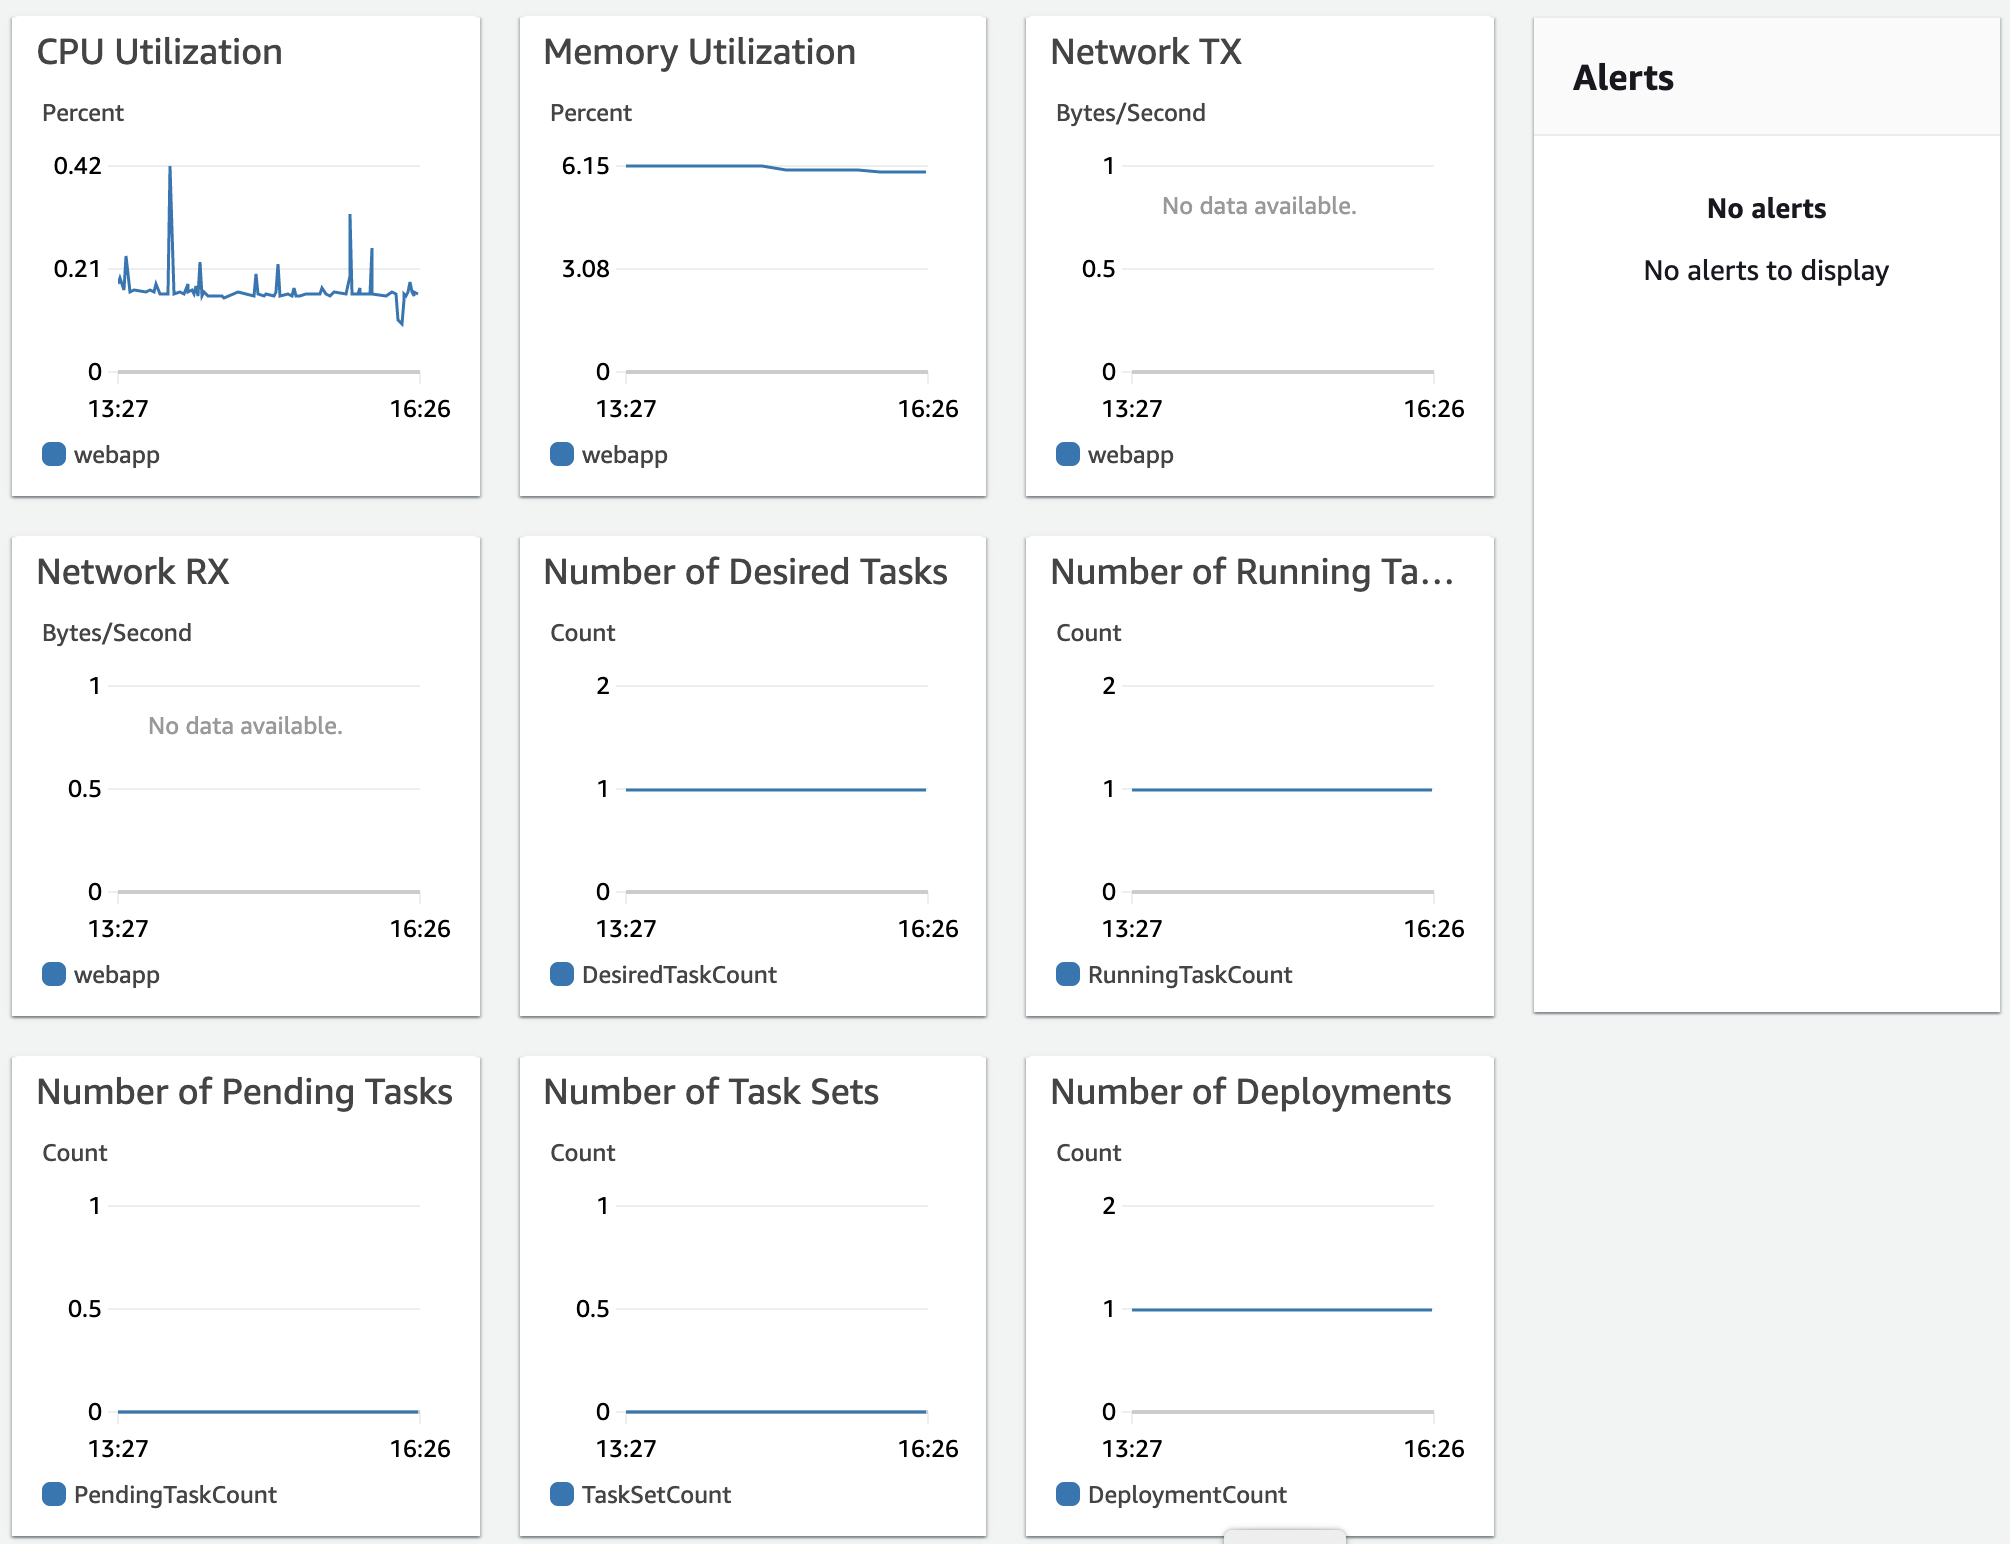
\includegraphics[width=0.70\textwidth]{pics/monitoring.png}
 \caption{Cloudwatch Monitoring Dashboard}
 \label{fig:monitoring}
\end{figure}
Another service we introduced in Chapter 3 is AWS lambda. It is the most important serverless service in AWS. We also discussed how could it be used in our DevOps toolchain in which monitoring is one of the use cases. In our monitoring system, AWS lambda is used as an extension for CloudWatch, and we use it for 2 cases.
\paragraph[]{Auto-Scaling the ECS Cluster with Custom Alarm in Cloudwatch}
As we mentioned in \ref{fig:deploy} Deployment Environment, The deployment could be auto-scaled by defining the auto-scaling policy within the ECS cluster. However, the scaling policy is not flexible enough; it only based on thresholds on certain metrics such as CPU utilization and memory utilization. Such auto-scaling in practice is: When the watched resources utilization is above/below a certain threshold, an alarm in Cloudwatch will be triggered. The alarm will further trigger the scaling event if the scaling policy was being set before.
\par
Nevertheless, in real-life development, many projects are microservices architecture, rather than homogeneous architecture as we have in the case project. According to Luca Tiozzo's article \cite{AWSECSho47:online}, this means some service (container instance in ECS) could be CPU intensive while the others might be RAM intensive. In such a situation, with Cloudwatch alarm based scaling, we need two groups of alarm watching RAM and CPU, respectively. Nevertheless, the problem is, when the ECS cluster lack of CPU resource but lack of RAM recourse, the CPU alarm is triggered then the ECS scaled up. Now the ECS cluster has enough CPU recourse, but it may have too much RAM resource so that it triggers the scale-in alarm in RAM. So the cluster will scale in again. This will cause the cluster to keep scaling up and back without finding and suitable size.
\par
A good practice solves the problem is to use a single group of alarm that only triggered by single metrics. We can set an AWS lambda function that read different metrics and then aggregate it to a single custom metric. The threshold and function that are aggregating the metrics need to be determined by the DevOps team according to the deployed project. Once the aggregated metric reach the threshold, the lambda function triggers an alarm that can trigger the scaling of ECS cluster. 
\paragraph[]{Custom Project-Specific Metrics}
The second application scenario is related to the first one. The Cloudwatch has support on recourse utilization metrics. However, some metrics are project-specific and not related to resources utilization and performance. For example, the number of successful payment has been made in a payment service. In such a case, Lambda could fill the gap within the scope of CloudWatch. The team could set up a Lambda function which gets the number by monitoring the log with PutMetricData provided by CloudWatch. This Lambda can further forward the metrics to metrics analysis and visualization platform, for example, Grafana \footnote{https://grafana.com/grafana/} to give the management team an overview of the KPIs.
\section{Design of Serverless DevOps Toolchain}
AWS provides a set of serverless DevOps tooling which could help us build a completely serverless DevOps toolchain. We introduced these tools in Chapter 3. In the section, we introduce the design of Serverless toolchain based on DevOps tooling of AWS. A certain part of the toolchain is the same with the non-integrated DevOps toolchain that introduced in the last section. Therefore we will not introduce these components again. Rather we only focus on how do we make use AWS DevOps toolchain. Figure \ref{fig:codepipeline} shows the general workflow of a project delivered by our serverless DevOps toolchain.
\begin{figure}[h]
 \centering
 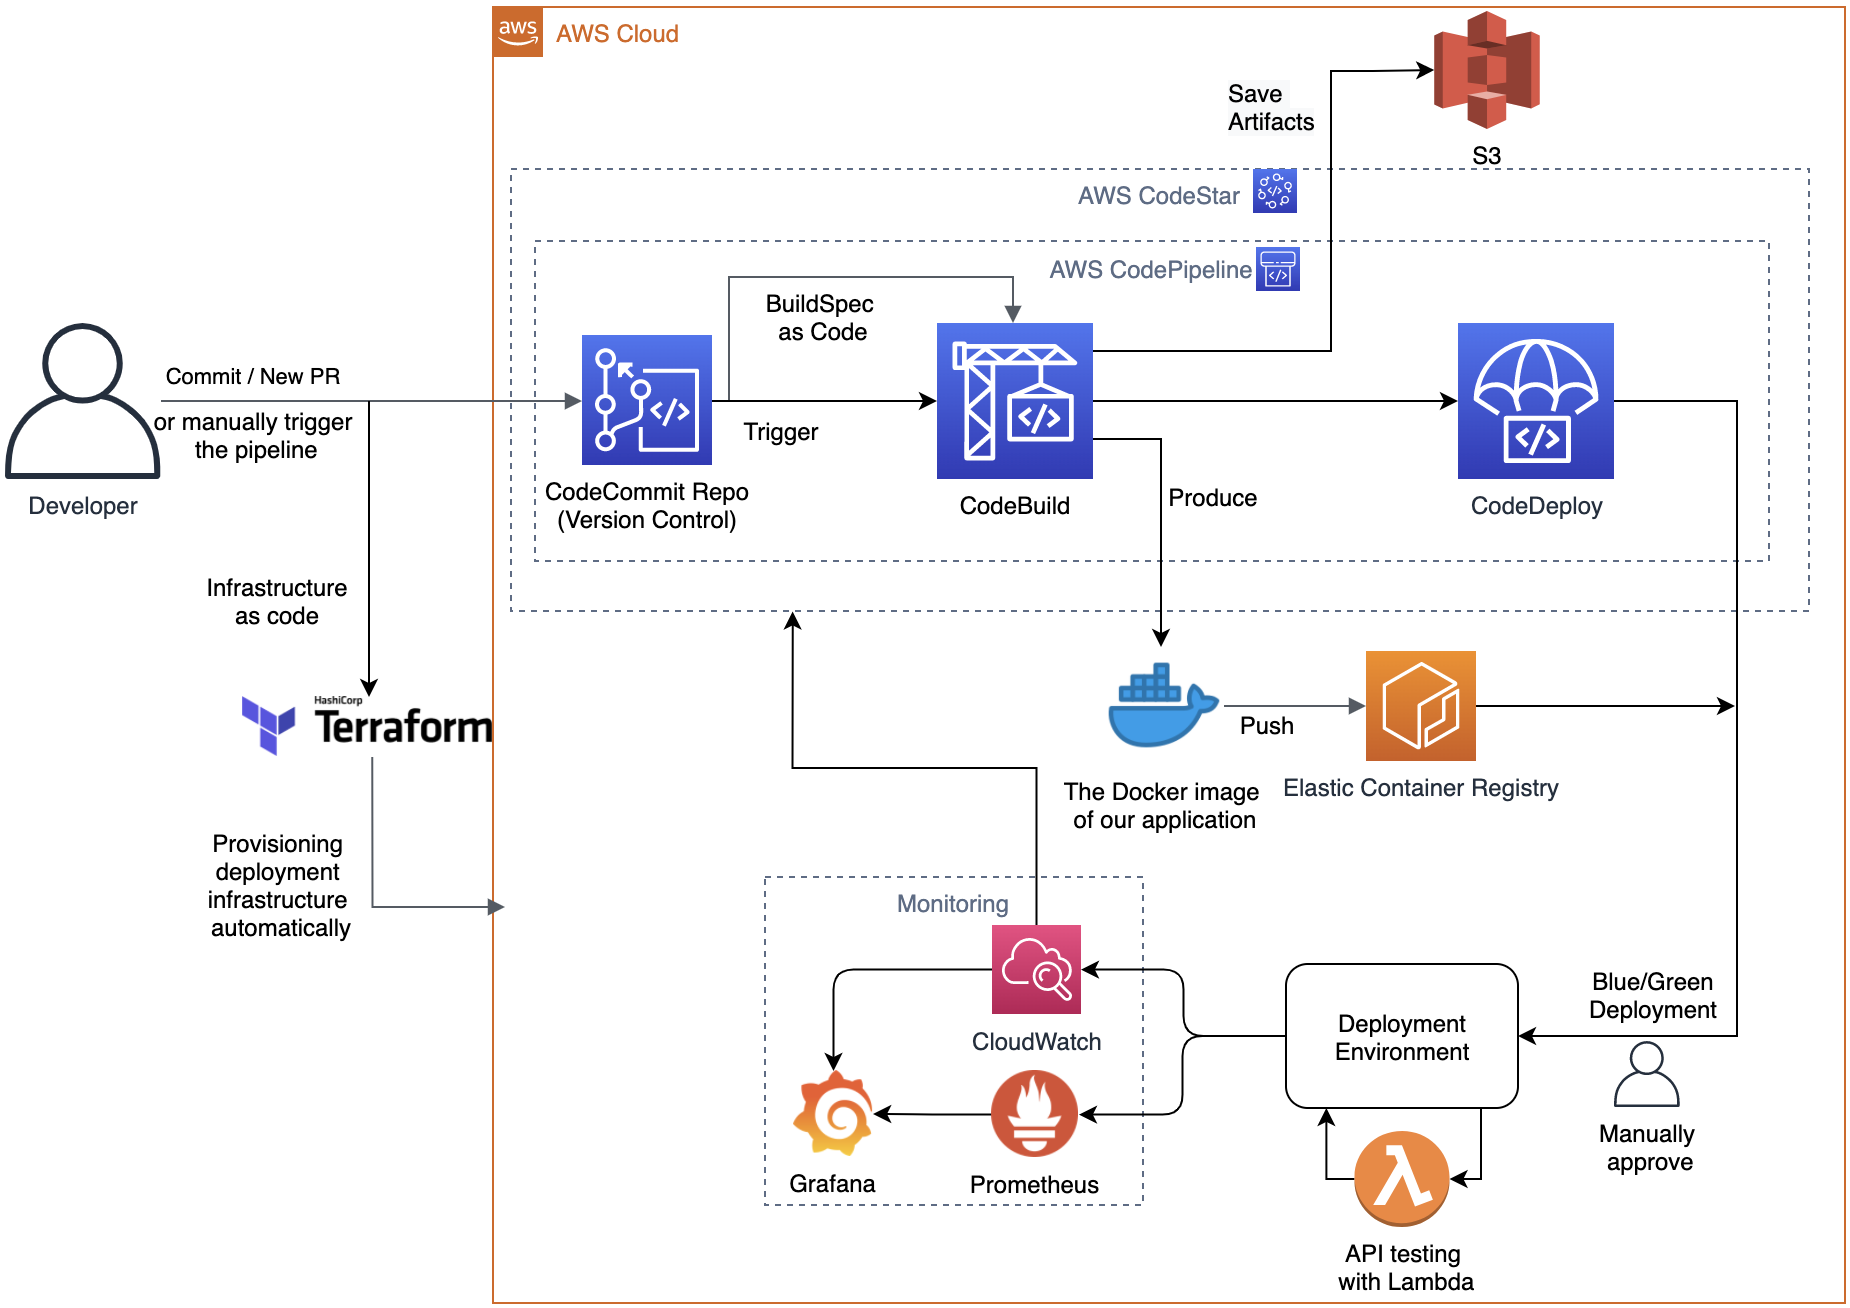
\includegraphics[width=0.90\textwidth]{pics/codepipeline.png}
 \caption{Serverless DevOps Toolchain}
 \label{fig:codepipeline}
\end{figure}
\subsection{Continuous Delivery Pipeline with AWS CodePipeline}
The workflow of our continuous delivery pipeline is the same as the pipeline in \ref{CD}. Instead of Jenkins, which is server-based, we build the pipeline with AWS CodePipeline. Figure \ref{fig:codepipeline} shows the activity within the CodePipeline in a single graph. Different from Jenkins who can do the whole continuous delivery process solely with the help of plugins, the CodePipeline just provides a platform which the development team can configure a workflow with AWS DevOps tooling or other third-party tools. 
\par
Same within the non-integrated version, we used GitHub as the version control system, and it has the same role as it has in the non-integrated toolchain. Although AWS also provides version control solution which is CodeCommit. It still lacks the functionality of collaboration compared with GitHub. Also, GitHub is already a serverless solution with good integration with AWS DevOps tooling, so we do not need to change our version control system away from GitHub. 
\par
In the next step, we are using AWS CodeBuild, which we introduced in Chapter 3. AWS CodeBuild does the same procedure as in Jenkins pipeline. It does code analysis, unit test and builds the Java application with Gradle, build the Docker image of the application and push to the ECR. Different, the cloud deployment deploys our application to ECS with Blue-and-green deployment strategy.
\par
The implementation of continuous delivery in CodePipeline is straightforward compared with Jenkins. In Jenkins, without the help of the plugin, the pipeline workflow can only be defined by groovy code, while CodePipeline natively provides a graphical user interface for workflow modelling. In our implementation, we just simply add each step with the graphical interfaces in CodePipeline.
\begin{figure}[h]
 \centering
 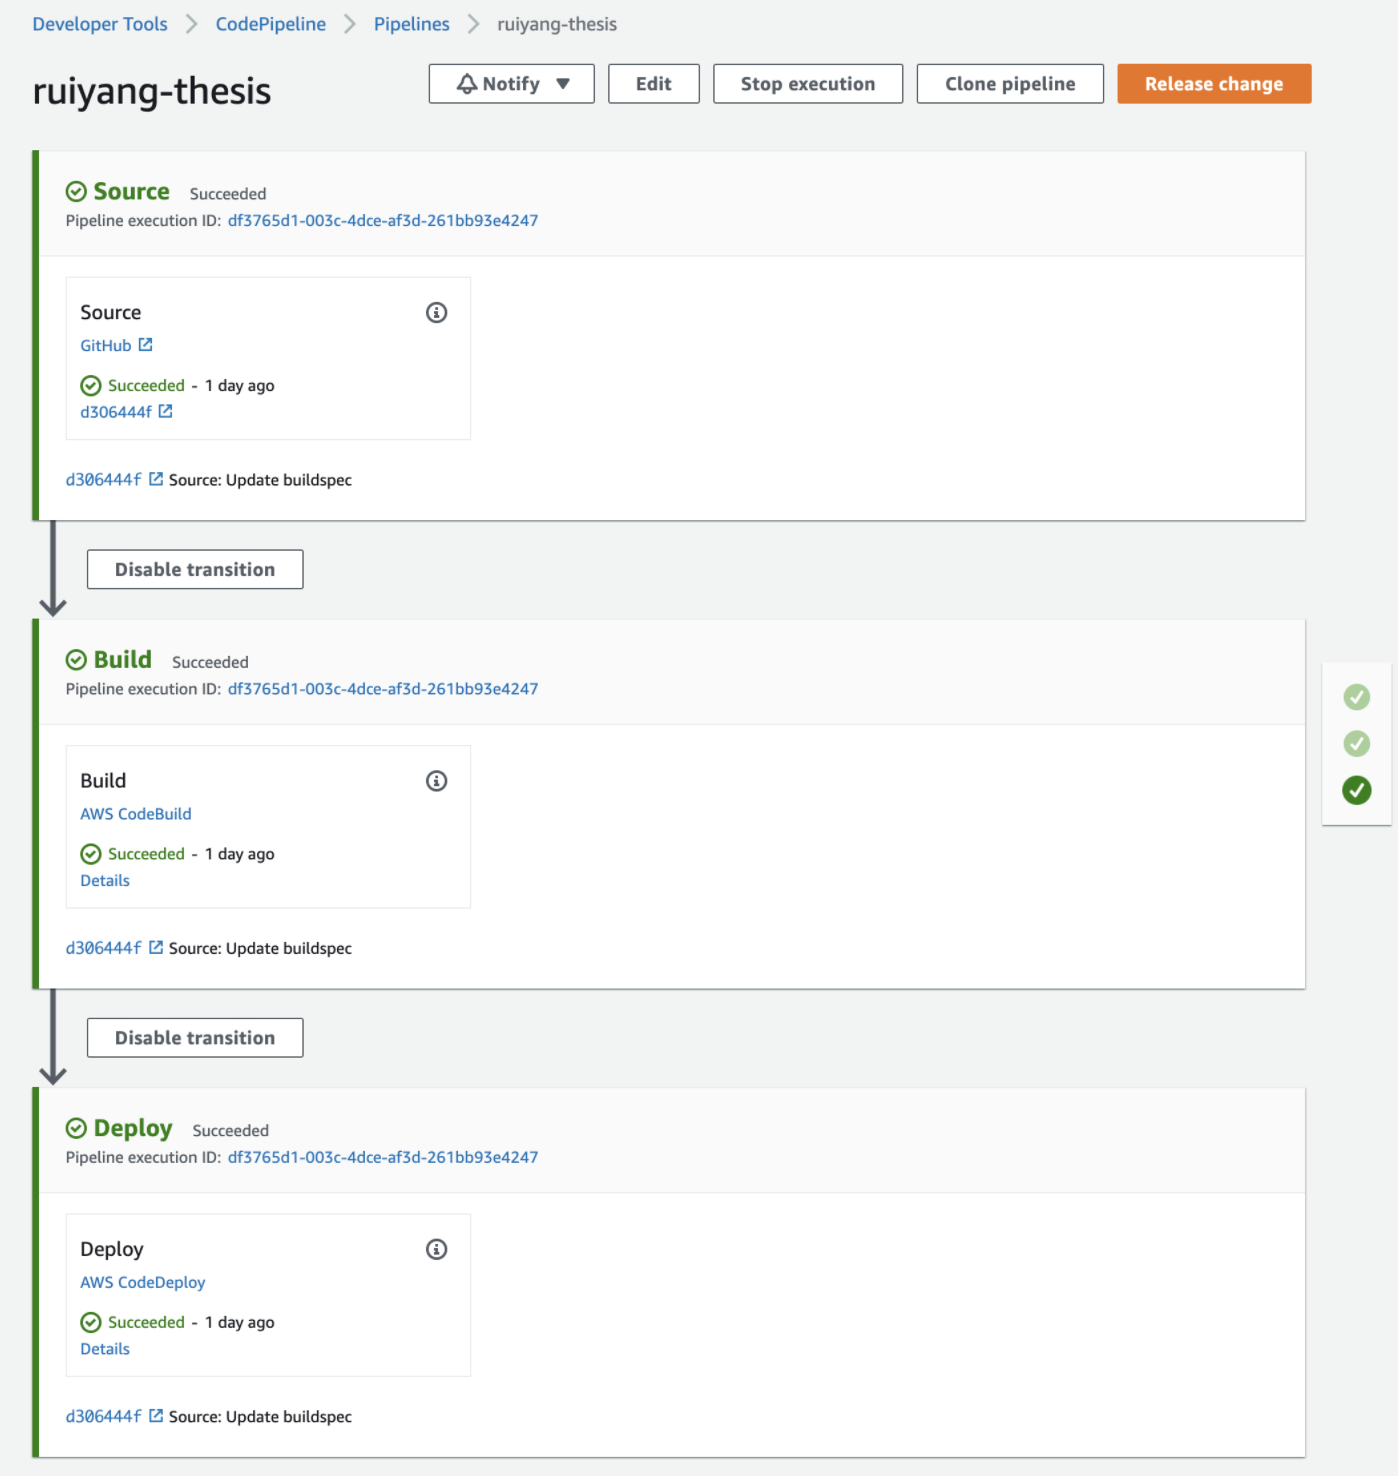
\includegraphics[width=0.75\textwidth]{pics/cp-interface.png}
 \caption{Our Workflow in CodePipeline}
 \label{fig:cp-edit}
\end{figure}
\subsection{Build and Test with AWS CodeBuild}
Same with the design of our Jenkins pipeline, AWS CodeBuild also executes the build within Docker container. The image of the Docker container provided by AWS already contains environment for the build of different programming languages. It also includes the Java environment and Gradle which needed by our case project. Therefore we could save time in setting up the pipeline since we do not need to define the Docker image for the build by ourself.
\par
As we mentioned in 4.3.1, the process within CodeBuild is the same as we have in Jenkins before the stage "Deploy". We will not describe the process again here. Same with Jenkins, the workflow of CodeBuild is defined in a YAML configuration file. The only difference in term of build workflow CodeBuild is that we store the build artifact to S3, the build artifact is the configuration file defines the deployment configuration in CodeDeploy. This is because CodeDeploy requires the deployment configuration from the step before it to run automatically.
\subsection{Blue/Green Deployment with AWS CodeDeploy}
One of the advantages of AWS DevOps tooling is good integration with other AWS services. During the design and implementation of our toolchain, this advantage shows in the deployment to ECS with CodeDeploy.
\par
In Jenkins, there is a lack of specific plugin that helps us deploy the project into ECS or EKS. Thus we have to deploy our project to ECS with AWS command-line interface(CIL). The problem with AWS CIL is that it only supports the most basic deployment strategy, which is rolling update deployment. The rolling deployment strategy is to replace the old code running on the instances with new code gradually, instance by instance. 
\begin{figure}[h]
 \centering
 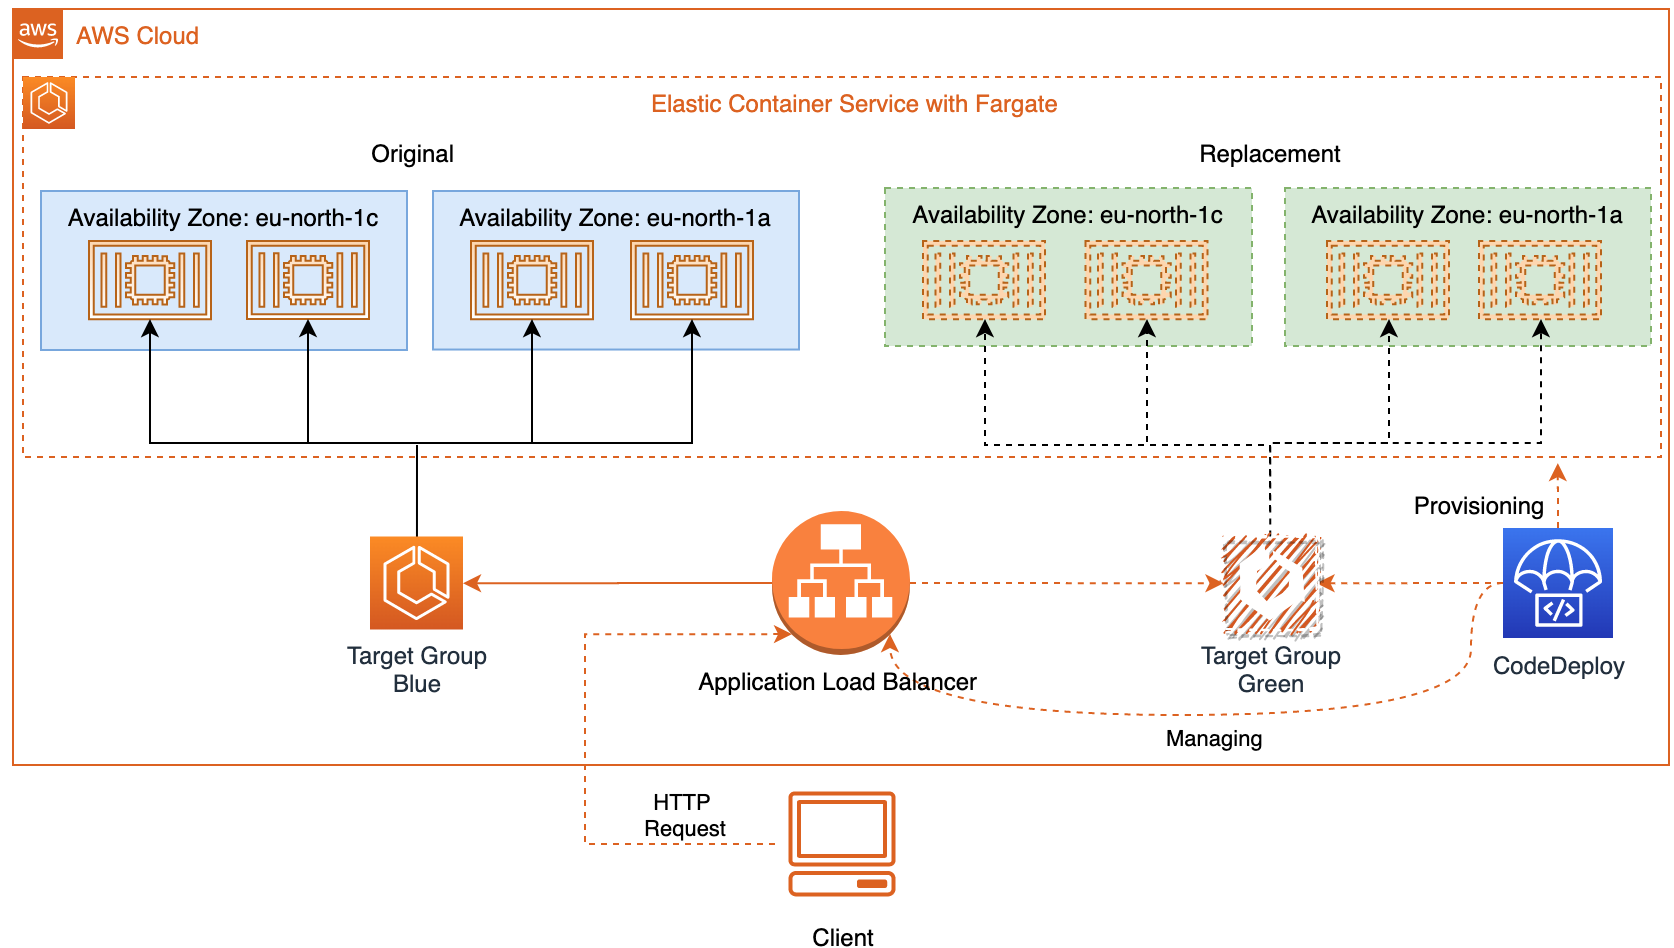
\includegraphics[width=0.99\textwidth]{pics/bg.png}
 \caption{Blue and Green Deployment for Our Deployment Solution}
 \label{fig:bg}
\end{figure}
\par
In real-life production, the team would like to make sure the deployment is reliable with minimized downtime. Thus the safety is highly valued in deployment strategy. In answering this need, a strategy called blue/green deployment, which is now widely used in the industry. AWS CodeDeploy natively supports the blue/green strategy.
A blue/green deployment is a deployment strategy that requires two sets of totally identical deployment environment that runs the new and original version of code respectively, while the router is gradually routing more incoming requests to the environment that runs the newer version of code. 
\par
Figure \ref{fig:bg} shows the visualisation of blue/green deployment. It also shows our design on how to implement blue/green deployment with CodeDeploy (shown before in Figure \ref{fig:deploy}). CodeDeploy controls a router before the load balancer. When new deployment comes, CodeDeploy does the following steps:
\begin{itemize}
 \item Provisioning new identical deployment environment (replacement environment) and deploy a newer version of code on it. In ECS, the deployment is called "task set".
 \item Control, the router, rerouting incoming traffic gradually to replacement ECS task set. We set the rerouteing rule as 10\% per minuets. We do not rerouting all traffic at once to ensure the service will not fully down if the new deployed task set not works properly. This minimizes the downtime of our deployment.
 \item Wait for 5 minutes after rerouting is done. During the rerouteing and this 5 minutes, the load balancer in replacement deployment environment keeps doing the health check by sending a request to health check API endpoint of our case project. CodeDeploy read the health status from the load balancer. If the replacement tasks set is un-healthy, CodeDeploy does rollback by rerouting incoming traffic back to origin tasks set.
 \item If the new deployment is still healthy after 5 minutes of waiting time, CodeDeploy terminates the origin tasks set. Now the whole deploy process is done.
\end{itemize}
Compare with the rolling update we are using in Jenkins pipeline, the better safety of blue/green deployment reflected at, when the error happens with a newer version of code, we can immediately roll back to the last version by switching the rerouteing to Blue \cite{UsingBlu65:online} without redeploying the previous version. Under the same circumstance, the rollback with the rolling update is nevertheless taking a too long time, since we have to replace the already deployed code to the previous version. This could cause longer downtime of the server. 
\begin{figure}[h]
 \centering
 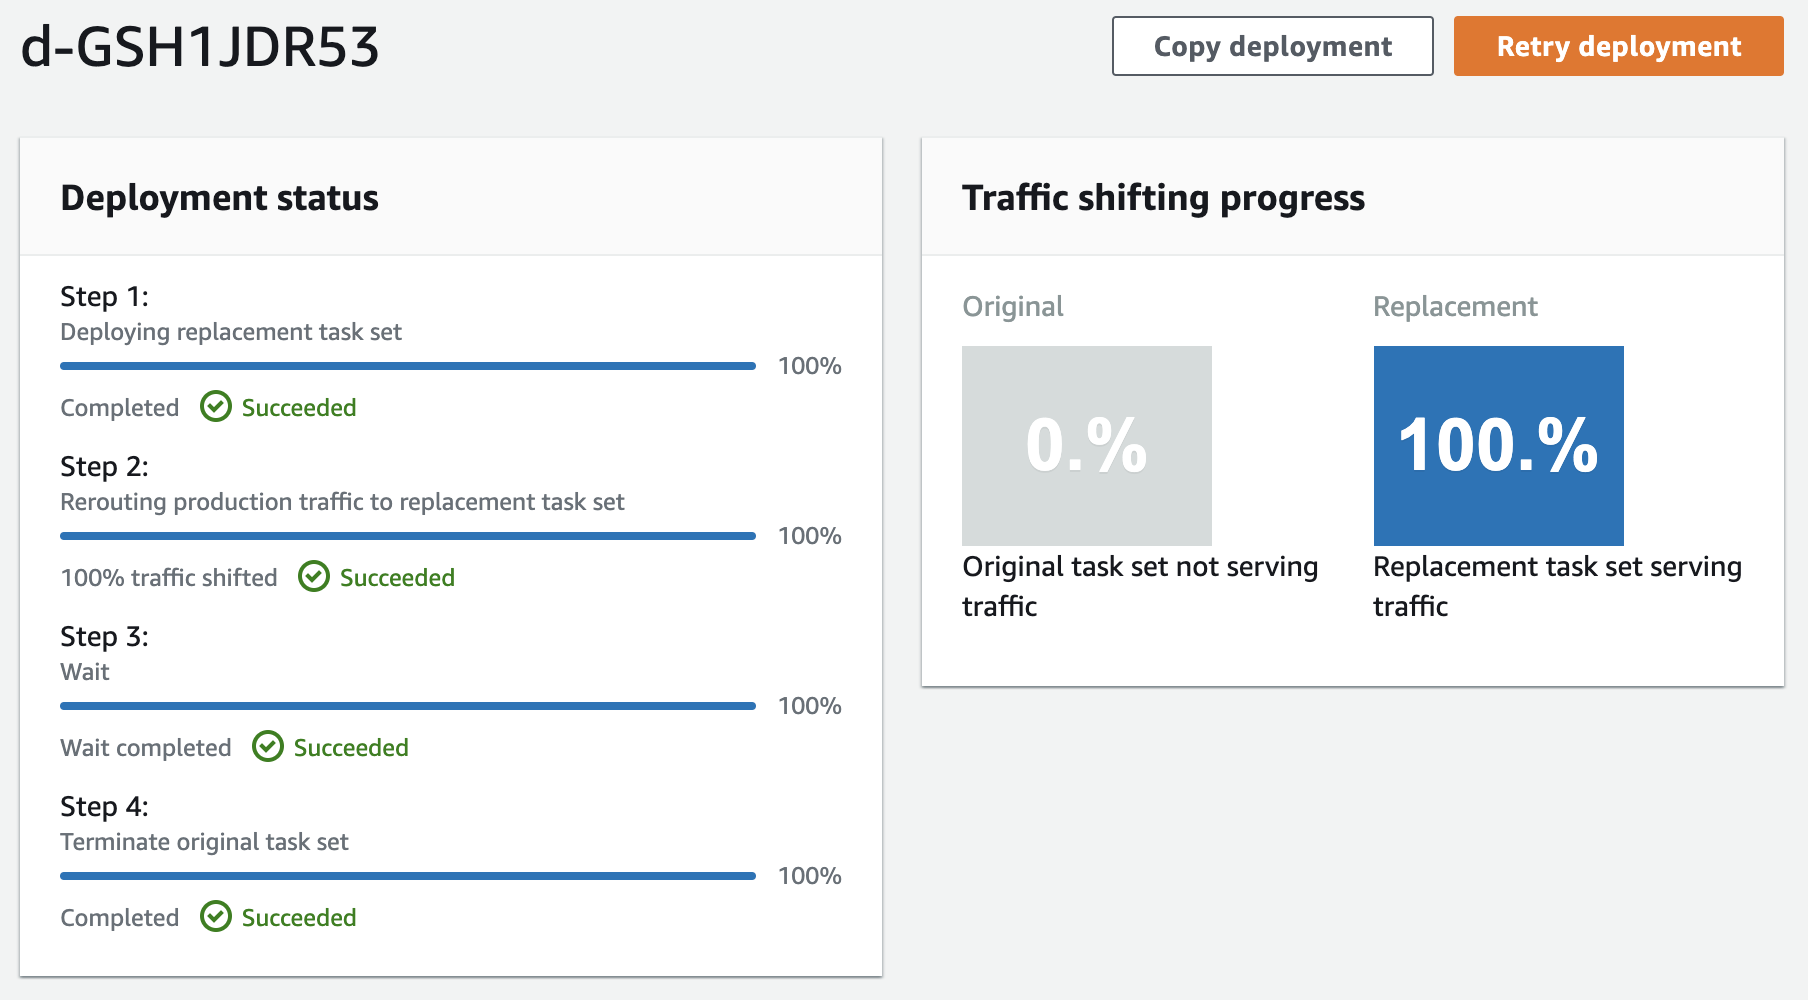
\includegraphics[width=0.90\textwidth]{pics/codedeploy_steps.png}
 \caption{CodeDeploy Dashboard}
 \label{fig:codedeploy_steps}
\end{figure}
\par
The better integration of CodeDeploy with the rest of AWS also be evidenced by the monitoring of the deployed solution. Aside from the existing monitoring with CloudWatch, CodeDeploy also provides us with a dashboard to show the deploy progress and the traffic rerouting process. Figure \ref{fig:codedeploy_steps} shows the dashboard of CodeDeploy that shows the status of our case project during the deployment.
% In comparison, with Jenkins + AWS CIL, we can not easily do the blue/green deployment. 
% \section{Cloud Services}
% \label{assumption}
% In this section, we will introduce several could service from CH3 that could be helpful to the DevOps toolchain. 
% //  Using services in AWS as an example, Introduces how cloud services could improve. describe services in one section
% \subsection{Managed Container Services for Distributed Builds} 

% // Describe how AWS Fargate could Help
% \subsection{Serverless computing}
% // Describe how AWS lambda could Help and why do we choose it
% \subsection{...}
\subsection{Integration of AWS DevOps Tools using CodeStar}
In 4.3.1, we introduce how do we integrate different stages in the continuous delivery pipeline (CD pipeline) with CodePipeline. However, an integrated continuous delivery pipeline is not called integrated toolchain. The DevOps toolchain is centred with the continuous delivery pipelines, but the pipeline is not all of the toolchains. To integrate other AWS tools with the CD pipeline and get the integrated toolchain as a single application, we use CodeStar.  
\par
Figure \ref{fig:codestar} show the user interface of the CodeStar dashboard. We can see, besides the CodePipeline, the CodeStar also integrate tools like monitoring, project management, and version control and then compose our integrated toolchain. In conclusion, the AWS integrated toolchain includes the following tools:
\begin{itemize}
     \item \textbf{CodeStar}: Integrate below tools into a signal toolchain. With project management functionality. The project management could be extended by integrating with third-party tools, i.e. Jira.
          \item \textbf{CodePipeline}: Modelling Continuous Delivery Workflow, integrate tools that used within the CD pipeline.
          \begin{itemize}
               \item \textbf{CodeBuild}: Build code of the software project.
               \item \textbf{CodeDeploy}: Deployment and monitoring.
               \item \textbf{GitHub}: Version control.
          \end{itemize}
          \item \textbf{CloudWatch}: Monitoring deployed solution.
\end{itemize}
\begin{figure}[h]
     \centering
     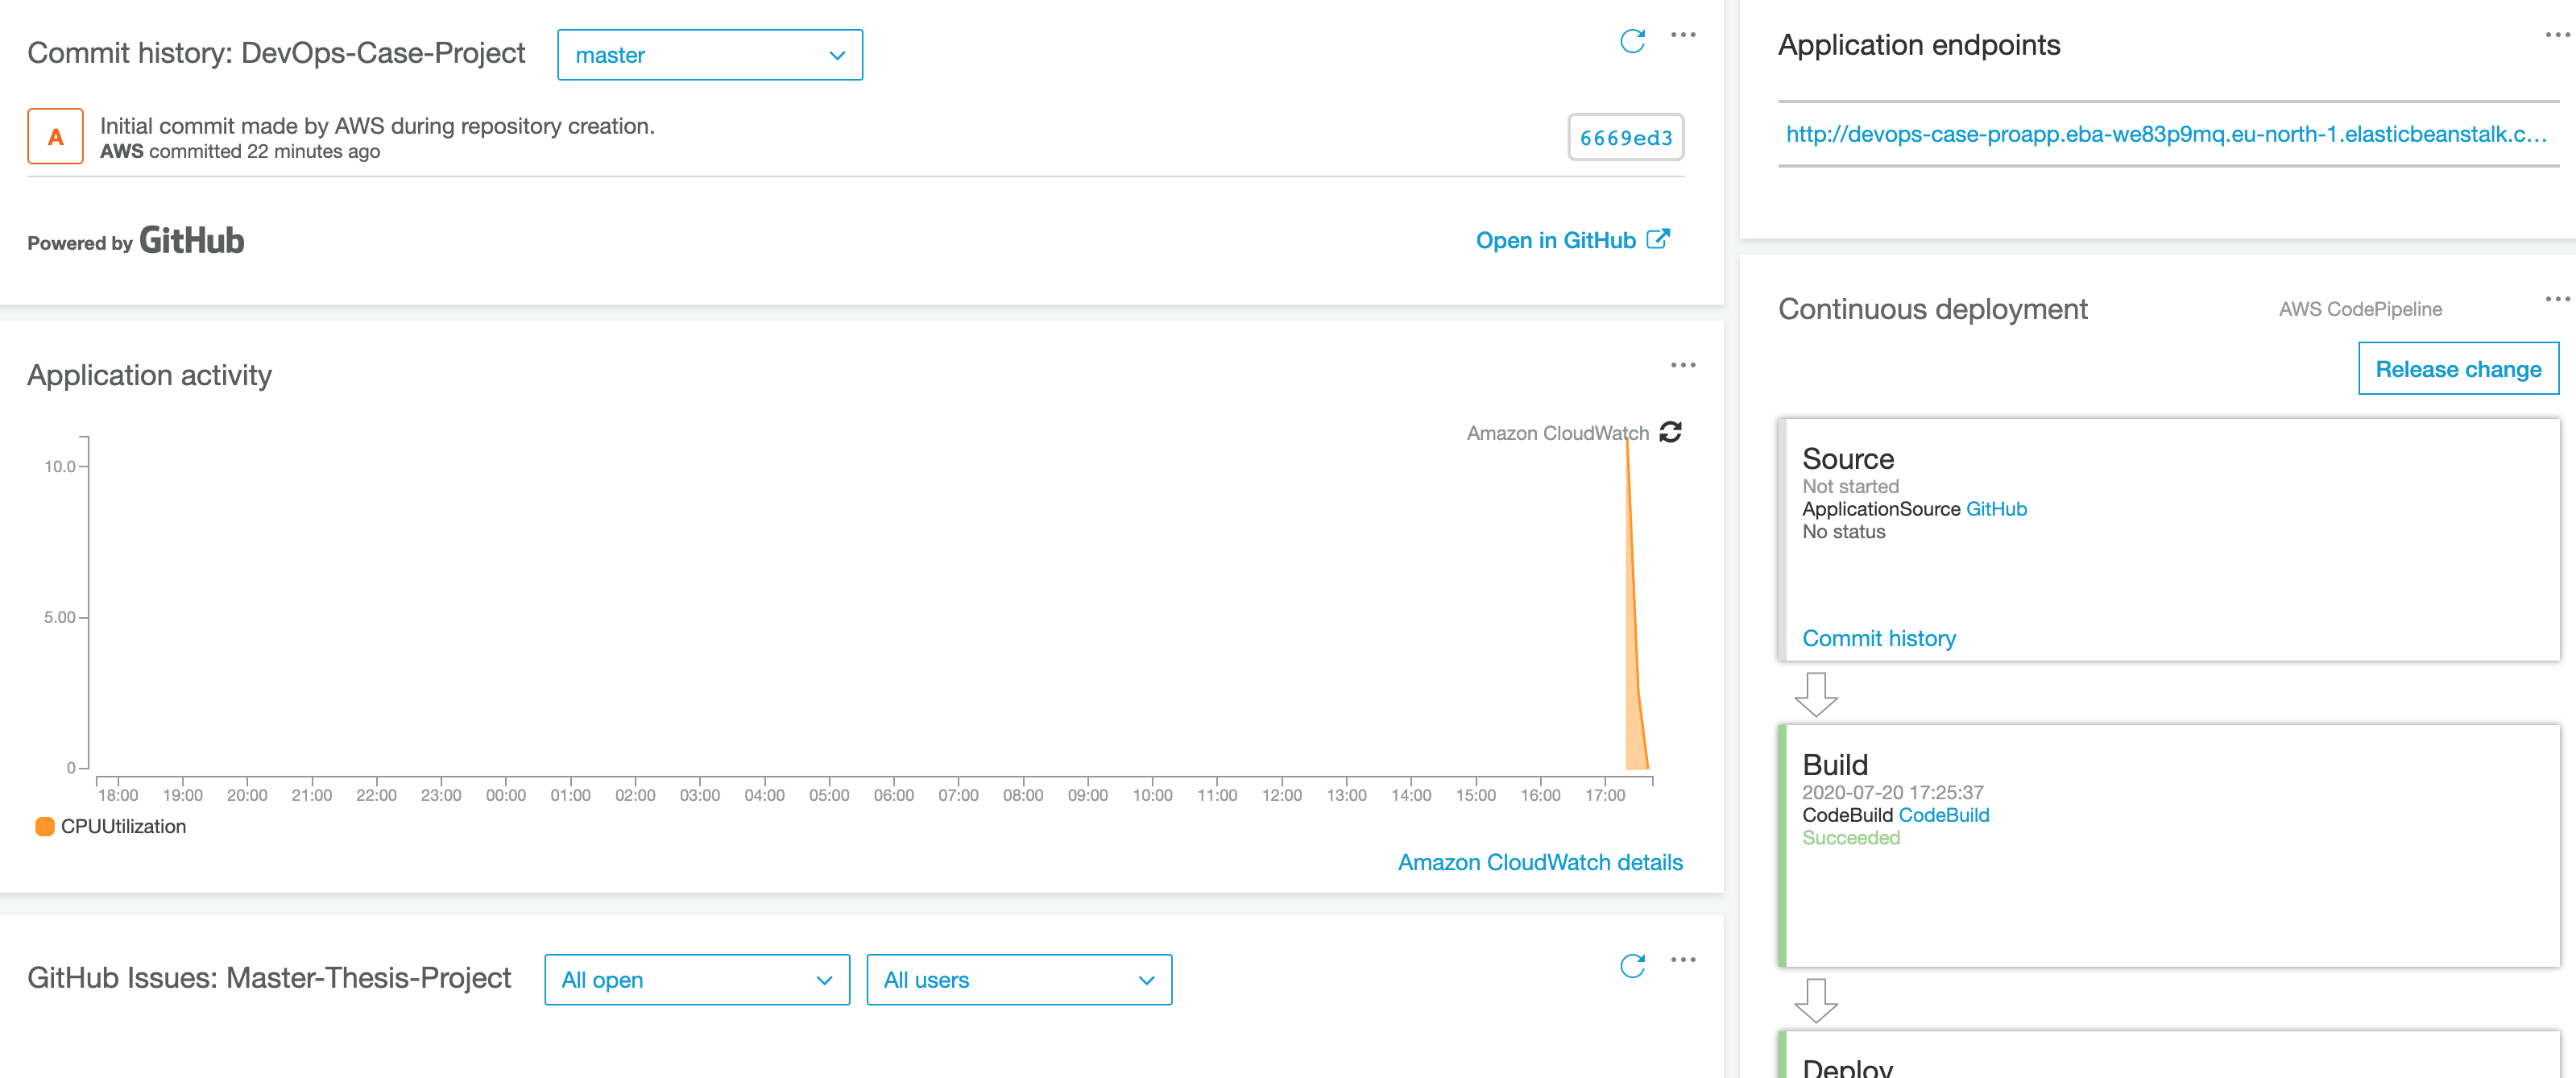
\includegraphics[width=0.99\textwidth]{pics/codestar.png}
     \caption{CodeStar Dashboard}
     \label{fig:codestar}
    \end{figure}

\section{Comparison between Integrated and Non-integrated Toolchain}
In this section, we discuss the difference between these two kinds of toolchains. The scope of comparison will be limited within the scope of functionality and ease of implementation. Furthermore, it is only based on our experiences with the tools used in our implementation.
We summarize the difference between these two toolchains as in Table \ref{tab:toolchain}.
We will do more comparison related to the performance and cost in Chapter 5.
\begin{table}[h]
 \centering
 \begin{tabular}{|c|c|c|}
 \hline
 &
 \begin{tabular}[c]{@{}c@{}}Non-Integrated \\ Toolchain\end{tabular} &
 \begin{tabular}[c]{@{}c@{}}Integrated \\ Toolchain\end{tabular} \\ \hline
    Open-source &
 \begin{tabular}[c]{@{}c@{}}Open-source solution\\ existed\end{tabular} &
 \begin{tabular}[c]{@{}c@{}}No, usually hosted \\ commercial solution\end{tabular} \\ \hline
 \begin{tabular}[c]{@{}c@{}}Delivery \\ method\end{tabular} &
 \begin{tabular}[c]{@{}c@{}}Each part is a stand-alone \\ tool either hosted or\\ on-promised,  depends \\ on the tools selection\end{tabular} &
 \begin{tabular}[c]{@{}c@{}}As a single cloud \\ hosted software\end{tabular} \\ \hline
 \begin{tabular}[c]{@{}c@{}}Implementing \\ time\end{tabular} &
      Long &
      Short \\ \hline
 \begin{tabular}[c]{@{}c@{}}Operational \\ effort\end{tabular} &
      High &
      Low \\ \hline
 \begin{tabular}[c]{@{}c@{}}Visibility \\ on status\end{tabular} &
 \begin{tabular}[c]{@{}c@{}}Depends on tools, a \\ well-integrated toolchain \\ could gives good overview\\ on the whole toolchain.\end{tabular} &
 \begin{tabular}[c]{@{}c@{}}Easy to see the\\ status as a whole\\ without additional \\ implementation\\ effort, low visibility\\ on under-laying \\ server since it's \\ hosted solution\end{tabular} \\ \hline
 \begin{tabular}[c]{@{}c@{}}Extendibility\\ and tool \\ selection\\ freedom\end{tabular} &
 \begin{tabular}[c]{@{}c@{}}Free to select tools\\ for each part of the\\ toolchain.\end{tabular} &
 \begin{tabular}[c]{@{}c@{}}Limited integration\\ with third-party \\ tools\end{tabular} \\ \hline
 \end{tabular}
 \caption{Comparison of continuous delivery tools}
 \label{tab:toolchain}
 \end{table}
\subsection{Implementation and Cloud Deployment}
The cloud based integrated toolchain is delivered as hosted solution in a serverless model. However we noticed that the non-integrated toolchain could be also completely serverless if we using hosted tools for all the components. 
\par
For example in our solution, we only have continuous integration pipeline which is on-promised and need to be deployed to the VM manually. If we replace Jenkins with some other hosted tools, for example, Travis CI\footnote{https://travis-ci.org/} we can actually build a fully hosted but non-integrated DevOps toolchain. But, for following reasons, it is not a satisfactory solution thus a non-integrated toolchain usually has some on-promised modules that needs operational effort and cloud knowledge.
\begin{itemize}
 \item The hosted tools, especially tools for continuous integration pipeline, are all closed-source commercial solution. This means there is no community support like in Jenkins, and it can usually integrates with the certain tools that supported by vendor. Besides, commercial user always need to pay for these hosted tools.
 \item Hosted tools runs in the vendor's server, and it requests user log in to use this tool which brings extra integration difficulty. This means for two hosted toolchain to integrated with each other, it not only need to do the integration in the data transfer, but also need to connect their account system, for example, with OAuth. This extra inconvenience makes most hosted DevOps tools only do the integration support with other most most popular tools which largely limited the extendibility.
\end{itemize}
Therefore, a non-integrated toolchain usually has some on-promised module in real-life use. In our deployment process, we find it requires lot of work to put an on-promised tool to cloud, especially if the developer is not familiar with the cloud platform that deploy this tools. For only deploying Jenkins we need to do following steps:
\begin{enumerate} 
 \item Create a cloud virtual machine (EC2 instances) for hosting the Jenkins master.
 \item Setup IAM role for Jenkins master VM, make sure it has access to other AWS recourse that needed during build.
 \item Setup security group and networking for the VM, makes sure it can be accessed form the internet but only accessible within company's IP range, and only port needed are opened to the public.
 \item Install Jenkins in the VM. Research what plugin is needed and install necessary plugins.
 \item An tedious set-up process for setup Jenkins cluster that supports the distributed build. This includes setup ECS cluster for build agent. Although Terraform makes the provision of cloud resources easier, still, prior knowledge for AWS is needed. The experiences in AWS is also needs to correctly configure ECS cluster that maximizing the performance of build agents.
 \item Develop Docker image for the container that runs Jenkins agents.
 \item Setup integration with other tools in toolchains by finding correct plugins and configure these plugins. 
\end{enumerate}
Only after these steps, we can start using Jenkins as part of our toolchain.
In comparison, the core feature of the integrated toolchain in AWS is an out-of-the-box feature which means there is no previous cloud knowledge needed, and there is no deployment and environment configuration required before we use it. We are free from all the steps we mentioned above.
\subsection{Extendibility and Flexibility}
The integrated toolchain is a hosted platform that runs by a vendor. Similar to we mentioned in 4.4.1, We find all the currently integrated toolchain are all commercial and closed-source which has no community support. So the integration of their third-party tools usually only limited to popular tools. For example, AWS DevOps tools only support 21 tools within it is "DevOps Partner Solutions" \footnote{https://aws.amazon.com/devops/partner-solutions/}. If the user wants to use anything except these tools, it is not possible.
\par
Nevertheless, different with the single hosted tools we mentioned in 4.1.1, a hosted integrated DevOps toolchain mostly has everything needed for DevOps lifecycle, so it is not mandatory for it to able to integrates with third-party tools. Still, the limitation in third party tool support might make the software team facing trouble when they want to use certain tools which are not very supported.
\par
A non-integrated toolchain allows the software team to pick any tools for each component, as long as those tools can be integrated. The tools in the toolchains could also be open-source, which allow so the software team modify the tools according to their need. For example, develop a plugin for Jenkins that allows the integration of internal company tool with Jenkins.
\par
In conclusion, in terms of extendibility and flexibility, non-integrated toolchains are better than integrated toolchain.
\subsection{Integration Between Tools}
As we mentioned in 4.4.1, sometimes it is hard for tools within a non-integrated toolchain to integrate, especially between the hosted tools. 
During our implementation, we also realized that, first, it requires some configuration work for tools to be able to work together. Secondly, sometime the Integrated could be buggy, for example, in our toolchain, the Jenkins sometimes does not react to the build triggering signal from GitHub. This means the software teams need further maintaining of the toolchain.
In integrated toolchain, the toolchains are delivered as a single cloud-based software, each part of naturally coped with each other, which makes integration much easier.
The better integrating between each component also makes it easier to monitor the toolchain as a whole.
\subsection{Visibility}
\label{visibility}
In 4.4.3, we mentioned that the integrated toolchain is easier to be monitored as a whole, however, when comes to every single component, in our implementation, we find out that integrated toolchain is lack of visibility. We met two difficulties when test two toolchain. The first one is that Jenkins master was having difficulty in the provision and connect to the agents. Since Jenkins is a web service deployed in our EC2 virtual machine, We solve the problem by reading the Error message within the Jenkins log file. The second problem we met was within AWS CodeDeploy. The CodeDeploy failed to deploy the case project to the ECS cluster. We could not find the reason at that time since we cannot find the log of CodeDeploy anywhere since it is not shown in the web interface, and we have no access to the underlying cloud infrastructure either. The lack of visibility is a problem with all hosted serverless services since the users do not have the visibility to the infrastructure behind the service.

\section{Challenges in Implementation and Design of DevOps toolchains}
In this section, we discuss the challenge that we met during the implementation. 
\subsection{Challenge I: The Enormous and Unregulated Jenkins Plugins System}
Jenkins has more than 1600 plugins which brings the software an amazing extendibility, which is one of the main advantages of Jenkins. However, there are two problems with Jenkins' plugins; First, there are usually more than one plugins that have the same functionality, for example, there are at least five different plugins related to running Docker container as Jenkins agent. Second, most of the plugin is developed by the open-source community, so the quality of these plugins is not ensured. During our implementation, we find out there are two plugins that support run Jenkins agent in ECS cluster. However, we find only one work after we tried both plugins. Besides, the documentation of Jenkins plugins sometimes is abysmal. For example, the documentation of the plugin that we use for Jenkins agent is too brief to tell us how to use the plugin, and it is not even mentioned the security setting needed in Jenkins master node that allows agents to connect the master node. 
\par
As a result of the above three factors, we spent a very long time in selecting and configuring tools. Moreover, trying to solve the problem which nether mentioned in the documentation and on the internet. 
\subsection{Challenge II: Fargate Does not Supports Container runs in Privileged Mode}
As said per title, this is some limitation in AWS Fargate for preventing container get permission to access the critical resource on the host(underlying server hosting Fargate instances in this case). As a result, we cannot use Docker within a Docker container that runs on Fargate. This makes it impossible for us to distribute the "Build docker image" and "Push to ECR" stages to agents. Instead, we have to run them on the master. Luckily, these two stages take a short time (<5s in total), so this limitation will not slow down the pipeline too much when multiple builds run in parallel.
\par
A possible solution solving this problem is to runs these two stages in AWS CodeBuild, AWS CodeBuild has support to Jenkins, which allow us to run certain Jenkins stages in CodeBuild. Moreover, CodeBuild supports fully parallel execution as in Fargate.
\subsection{Challenge III: Slow Starting Time for Agents in AWS Fargate}
On average it takes around 60s from sending a Jenkins job to agent, to running the job in an agent. To our case project that takes 90 seconds to go through the whole pipeline, this is a relatively long time. During this 60s, Jenkins master node sends task definition \footnote{Define specification of a container runs in ECS.} to ECS, provision a Fargate instance within ECS, then pull the image we developed for Jenkins agent, star the agent container within Fargate and then connect to the Jenkins master. This challenge is due to the nature of the serverless computing that we discussed in Chapter 2, and we believe there is not an economical way to solve the challenge with the current setup.
\subsection{Challenge IV: No Enough Visibility in AWS DevOps tooling}
As we mentioned in \ref{visibility}, the lack of visibility to the underlying process, especially in CodeDeploy, caused some obstacle for us to debugging our pipeline. There was a problem when we try to deploy the case project to the ECS with blue/green deployment, and the CodeDeploy sucked in the creating replacement service. We know there was something wrong within either the configuration of ECS, load balancer, health-check or security/network setting. Nevertheless, there is no log output of the underlying deployment process in CodeDeploy. In the end, we have to check everything that might be caused problem one by one and found it was the problem with failed health-check, which was very time-consuming.
\chapter{Performance Comparison and Evaluation}
In this chapter, we describe our experiments regarding two research questions we proposed in Chapter 1. The experiments based on the DevOps toolchains we implemented in Chapter 4.
\par
In Section 5.1, we will examine how does the serverless compute engine for containers (Amazon ECS on AWS Fargate) could influence the performance of non-integrated toolchains. Thus, in the experiment, we implement the solution with a different type of cloud environment (with/without serverless) as a comparison group.
In Section 5.2, we focus on answering research question 2, in which we will compare the performance of continuous delivery pipeline composed of fully-managed serverless DevOps tools in AWS with our Jenkins-based pipeline that runs on the virtual machine.
\section{Experiment 1: Experiment on Serverless Container Services}
The Docker agent has already been supported by many CI/CD tools ad we introduced in Chapter 4.
The serverless container services in AWS (AWS Fargate) provides the possibility to ease the infrastructure management task for the Docker build agents.
This experiment is a controlled experiment which examines whether serverless container service could improve the continuous delivery pipeline from various perspectives.
\subsection{Test Task and System Description}
In this experiment, we run the continuous delivery process of a Spring Boot web application with our DevOps toolchain. From the experiments, we could verify our assumption in Chapter 3 and better-answering RQ 1.
\par
As we described in Chapter 4, the continuous delivery pipeline includes the following steps:
\begin{enumerate}
\item \textit{Checkout}: Pull the most recent change from GitHub repository
\item \textit{Build}: Build the application with Gradle, with automating testing with JUnit integrated into Gradle.
\item \textit{Build the docker image}: Build the docker image of our Spring Boot application.
\item \textit{Push to Container Registry}: Push the docker image from the last step to the AWS elastic cloud registry (ECR) for further deployment.
\end{enumerate}
\par
In these four steps, the step "Build", and "Checkout" is being done in parallel within the ECS cluster. As we mentioned in CH4, when the new job started in the Jenkins master server, Jenkins will provision a new container instance within the ECS cluster. The container is managed directly by AWS, so we don't need to create and manage the virtual machine that runs the container. We use this setup in our initial implementation as the control group.
\par
In the experimental group, we replace AWS Fargate with traditional VM, which is EC2 in the Amazon Web Services.The parallelisation pattern remains the same; this means as in the control group, only the first two steps are being run distributively in the Jenkins nodes. The EC2 instances belong to an auto-scaling group that will scale up when CPU Utilisation rate reach 70\%. The initial size for an auto-scaling group is 1.
\par
Figure \ref{fig:ex1} shows the architecture of 2 groups in this experiment. The experimental group on the left is a Jenkins server with the traditional virtual machine as workers node that hosting the container agent. The architecture of the control group on the right has agent nodes dynamically provisioned as serverless containers hosed by AWS Fargate.
\begin{figure}[h]
\centering
\begin{minipage}{0.45\textwidth}
\centering
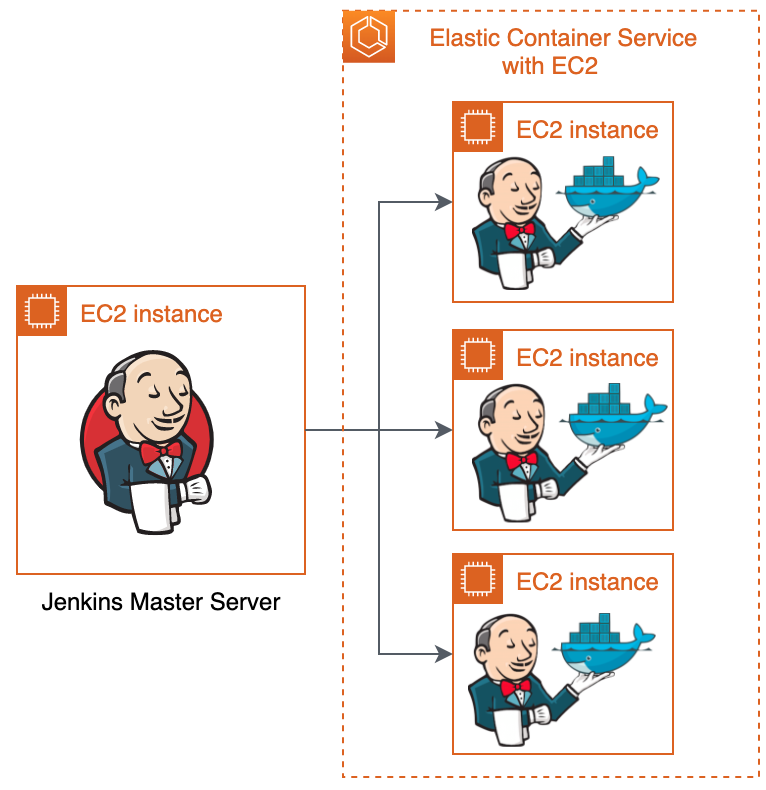
\includegraphics[width=\textwidth]{pics/jenkins-on-vm.png} % first figure itself
\end{minipage}\hfill
\begin{minipage}{0.54\textwidth}
\centering
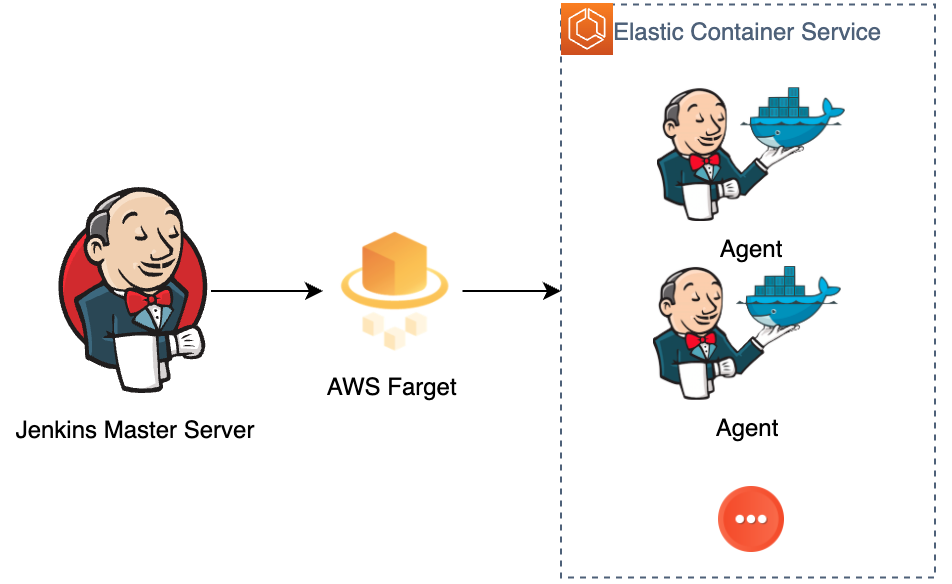
\includegraphics[width=\textwidth]{pics/jenkins-on-fargate.png} % second figure itself
\end{minipage}
\caption{Architecture diagram of the test Jenkins cluster with agents running in traditional virtual machines (left) and on ECS with AWS Fargate (right)}
\label{fig:ex1}
\end{figure}
\subsubsection{Hardware}
The hardware of the instance that runs Jenkins agents is the independent variable that exposed to the change in the experiment.
\par
The experiments are conducted on Amazon Web Services (AWS). The hardware of Jenkins master node in both experiment groups is the same, which is EC2 instance of type t3.medium with two virtual CPU, 4 GB RAM and 30 GB disk. The EC2 instances as worker node are type t3.small, with two virtual CPU and 2GB RAM. Each EC2 instance can run one container at the same time.
\par
In the control group, which is the implementation we presented in CH4, the Jenkins agents run on AWS ECS powered by AWS Fargate. The virtual hardware resources that are allocated to each serverless container is two virtual CPU, and 2 GB of RAM. The identical hardware setup between to groups makes sure that each container shares the same hardware resources as in another group, so the hardware will not affect the result.
\subsubsection{Software}
We maintain the same software setup in each group. The version of the software is all the latest version as for February 2020. The operating System for EC2 instance that runs Jenkins master node is Ubuntu Server 18.04. The version of Jenkins that runs on the server is 2.222.3. For connect ECS and Fargate which works as the Jenkins agents, we use Jenkins plugin "Amazon Elastic Container Service (ECS) / Fargate", version 1.34. The container in Fargate/EC2 for running the Checkout and Build steps is from our developed docker image, which can be seen at \footnote{https://hub.docker.com/r/dry1995/jnlp}. The docker image includes essential dependencies that will be used to build the Spring Boot application. It's the base image include a program which allows container connects Jenkins master as an agent. The "Build" step in our pipeline uses Gradle (version: 6.2.1) as the build tool for the application,
with OpenJDK 1.8.0.252 as Java virtual machine (JVM).
This step also includes the automated testing and code analysis, as plugins of Gradle. 
\par
To shows how does the two setups performance within the teams with different sizes, we run by run the different number of tasks parallel through the pipeline. This scenario simulates the different team size and shows the scalability when it comes to the need for task parallelisation in larger organisations. It also imitates the DevOps process of a microservices software project, which could have multiple jobs for different service runs in parallel.

\subsection{Performance Properties and Evaluation}
We run the pipeline through 2 different setups, and we will get the result of the following properties:
\begin{itemize}
\item \textit{Runtime} describes the total time for finishing all the jobs. If the jobs run in parallel, the runtime is from the start of jobs until the end of the last finished job.
\item \textit{Cost Structure} describes the daily cost of 2 setups under the same workload, within the same period.
\item \textit{Resource Utilisation} describes the average CPU/RAM usage for each instance during a single run of the pipeline. The purpose of this comparison is to show the performance of the same application in a different environment (EC2 and Fargate).
\end{itemize}
\subsection{Result and Evaluation}
Here shows the result of this experiment. We also evaluate our experiment result by analysing the factors that lead to the results.
\subsubsection{Runtime}
We first compare the runtime of these two setups. Except for test the runtime of single job runs with two setups respectively, we also test the runtime of each pipeline setup under different number jobs executed in parallel. Figure \ref{fig:runtime} shows the test result.
\begin{figure}[h]
\centering
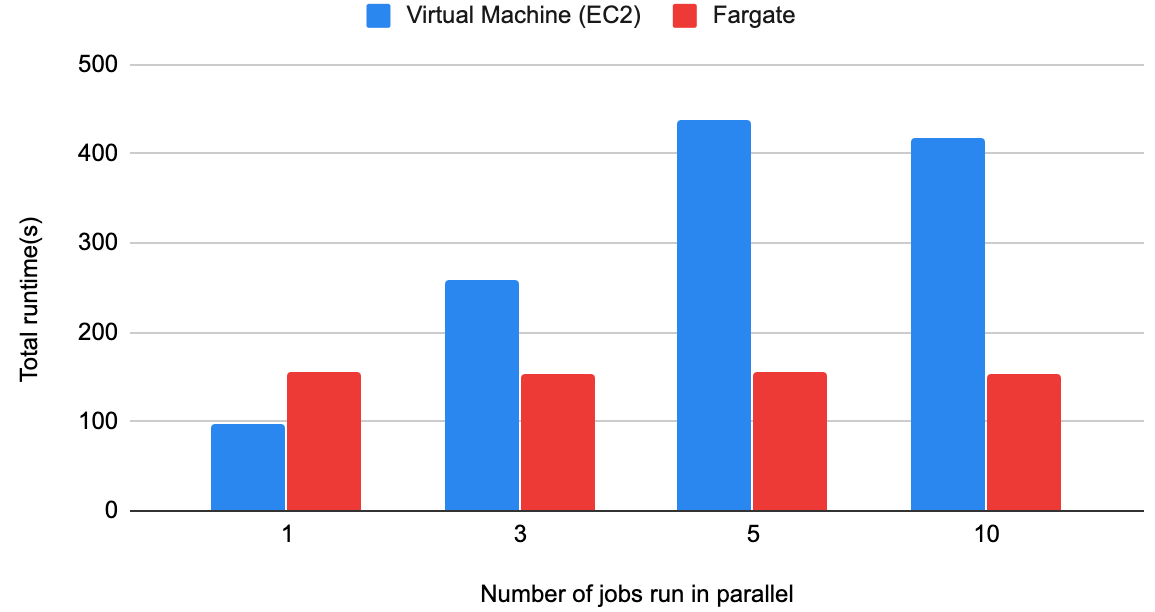
\includegraphics[width=0.99\textwidth]{pics/runtime.png}
\caption{Runtime of Pipeline with Different Jenkins Agents Under Different Number of Jobs Runs in Parallel}
\label{fig:runtime}
\end{figure}
\par
The test result shows that when it comes to the execution of a single task. The traditional VM has a faster delivery speed over serverless solution (AWS Fargate). However, with the number of jobs that run in parallel increases, the total runtime on the traditional VM decrease. On the contract, on the serverless solution(Fargate), the runtime remains almost the same.
\par
We analyse the reason behind this result, and we found out that the longer runtime with the single job on Fargate is because the longer starting time of Jenkins agent. In EC2, the Jenkins will simply provision a Docker container within EC2 VM, and connect to the Jenkins master node. However, in Fargate, the Jenkins can only connect to the agent once AWS finishes the initialisation of underlay infrastructure that runs the serverless container, which takes a significantly longer time. The slow provisioning shows one of the limitations of serverless computing (cold-start) that we mentioned in \ref{servlesslimitation}.
\begin{figure}[!h]
  \centering
  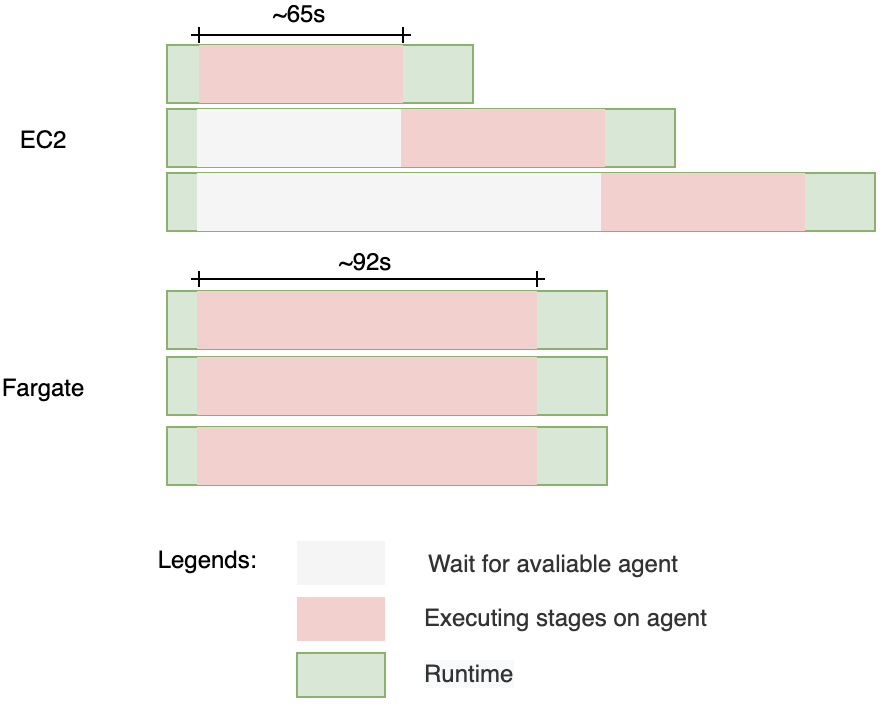
\includegraphics[width=0.90\textwidth]{pics/parallel.png}
  \caption{Execution Mode of Pipelines with Different Jenkins Agents}
  \label{fig:parallel}
  \end{figure}
\par
When it comes to parallel job execution, the performance of Fargate is significantly better. The performance difference is because, in Fargate, each container runs on an independent instance on AWS's infrastructure. Therefore, AWS provisions one Fargate instance for each running job. The independence between Fargate instance ensures the agent will not compete for the resource. On the other hand, when we run multiple agents in our EC2 instance, due to the limitation of resource, part of running jobs has to wait until the resource on EC2 instance available until they can start the execution. To further investigate the reason for the result, we observe the parallel execution mode when it runs three jobs in parallel. Figure \ref{fig:parallel} shows the execution modes. We find that the easily scalable character (mentioned in \ref{servlesslimitation}) helps the serverless suites better with the parallel task. The long wait time is the reason that makes the total runtime in EC2 much longer.
\par
We also notice that in Figure 5.2, when the parallel task reaches 10, the EC2 runtime becomes shorter. The shorter runtime of EC2 is because we set auto-scaling for our EC2 instance. So in the later part of our experiment, the EC2 scaled from 1 to 2 and then to 3. Nevertheless, even with 3 EC2 instances, only three jobs are allowed to run in parallel, while in Fargate is easy to have ten jobs runs in the complete parallel method. This because the scaling of EC2 VMs is much slower because it is heavier to create a VM than create a new Fargate instance. The other reason is the auto-scaling of EC2 VM is triggered by reaching certain resource utilisation threshold, but in Fargate is based on task number(Jenkins agent number). Even we set the scaling policy of EC2 to a more aggressive pattern, the AWS still more "hesitate" to create new instances compared within the Fargate. 
Therefore, in the real-life software development, when the number of jobs surges in Jenkins cluster, the Fargate could react faster in terms of scaling. And when the job drops, Fargate also scale-in faster, which saves cost.
\subsubsection{Resource Utilization}
We compared the average resource utilisation within containers that runs Jenkins agent in two setups. The data from the AWS CloudWatch (Figure \ref{fig:utilizationecs}) shows that the resource utilisation rate is similar in these two setups. The similarity is because the "run in the same way regardless of the host environment" \cite{WhatisaC60:online} feature of Docker container that we mentioned in \ref{docker}.
\begin{figure}[h]
\centering
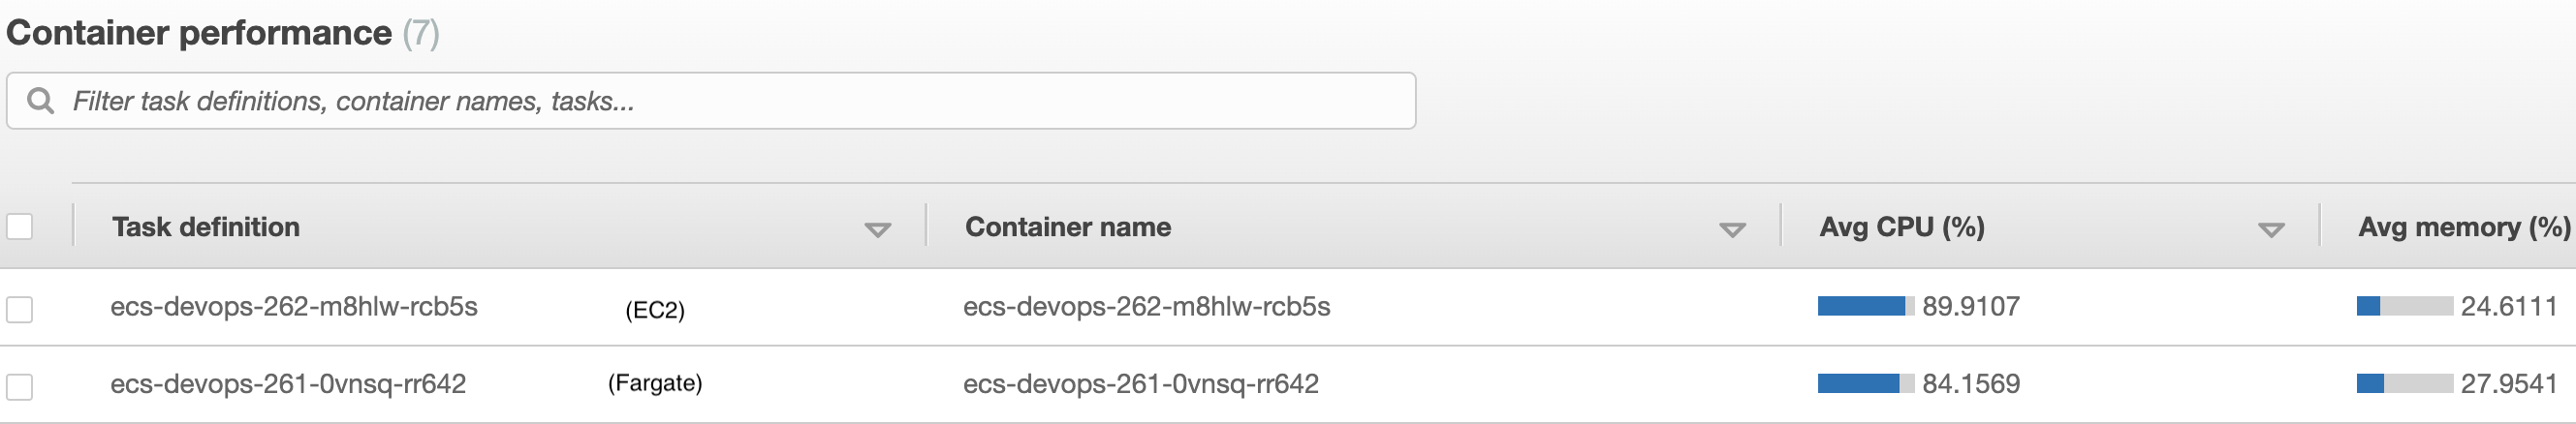
\includegraphics[width=0.99\textwidth]{pics/utilizationecs.png}
\caption{The comparison of Resource Utilization}
\label{fig:utilizationecs}
\end{figure}
\subsubsection{Cost Analysis}
The container orchestration service ECS itself is free of charge. We only pay for the resources we are using, which is Fargate or EC2 virtual machine.
\par
In AWS Fargate we pay only by resource we are using and the runtime. The price for Fargate service in EU(Stockholm) is \$0.04165 per GB RAM per hour plus \$0.0049 per vCPU per hour \footnote{https://aws.amazon.com/fargate/pricing/}. Thus, in our experiment setup (2vCPU, 2 GB RAM), the price should be \$0.0931 per running agent for one hour's runtime.
In AWS EC2 our cost depends on the type of VM we are using. The type of VM we use for running Jenkins agents is t3.small that costs \$0.0216 per hour \footnote{https://aws.amazon.com/ec2/pricing/on-demand/}. The Fargate-based Jenkins agent is more expensive than EC2-based agent.
\par
However, the pay-per-use characteristic of serverless service makes Fargate more competitive in terms of cost. The instance only up and run when Jenkins master distributes the job. Once the job finished, the AWS will terminate Fargate instance immediately when it finds no container is running on it. However, EC2 not so flexible due to the resource-utilisation-based scaling policy. The EC2 instance is not scaled in immediately after job finished, and the user has to pay for the instance runtime before it gets terminated -- even there is no job running in EC2 instance any more. So depends on the frequency and length of the build task, the user could have runtime per hour when using Fargate instance.
\subsection{Conclusion}
In this experiment, we compare the serverless (AWS Fargate) and non-serverless solution (EC2) for hosting distributed continuous delivery pipeline. The experiment shows that the performance of the serverless solution is worse when it comes to single job execution, which is because of the cold-start issue with serverless computing. However, in terms of the parallel job executing, the serverless solution has better performance over traditional VM. 
\par
\label{micros}
An better parallel execution performance is meaningful for apply DevOps practice in the microservices development. A microservices could have hundred of services. In the philosophy of microservices, the release of each service should be independently \cite{dehghani2018break}. To ensure this, one practices it to use one pipeline for each service. However managing a hundred pipelines is not an easy task, and better practice is to have multiple services share a single pipeline \cite{HowtoSca9:online}. Therefore, when multiple services share the same pipeline, this improvement allows services to be released independently without waiting for each other.
\par
In term of cost, the serverless solution is more expensive per hour. However, the difference could be offset by the less runtime. Moreover, resource utilisation is similar in both solutions. Table \ref{tab:exp1} show a comparison between two experimental groups.
\begin{table}[h!]
    \begin{center}
        \begin{tabular}{|l|l|l|}
        \hline
         &
          EC2 Agents &
          Fargate Agents \\ \hline
        Build Time &
          \begin{tabular}[c]{@{}l@{}}98s for a single task.\\ Largely increases when\\ run multiple tasks in \\ parallel\end{tabular} &
          \begin{tabular}[c]{@{}l@{}}155s for a single task.\\ Remains unchanged when\\ multiple task runs in \\ parallel\end{tabular} \\ \hline
        Cost &
          \begin{tabular}[c]{@{}l@{}}Lower per hour price\\ (\$0.0216)\end{tabular} &
          \begin{tabular}[c]{@{}l@{}}Higher per hour price\\ (\$0.0931), however the\\ billable hour is shorter,\\ the total price could be\\ lower.\end{tabular} \\ \hline
        \end{tabular}
        \caption{Conclusion of Experiment 1}
        \label{tab:exp1}
    \end{center}
        \end{table}
\section{Experiment 2: Experiment on Integrated DevOps Toolchain}
For solving the RQ2, we compare the implementation of our design of two different the DevOps toolchain -- the non-integrated Jenkins based toolchain and the AWS DevOps toolchain implementation with AWS DevOps tooling.
\subsection{Test Task and System Description}
This second experiment is similar to the first experiment, and we deliver our case project through two DevOps toolchains. The first toolchain is our Jenkins-based toolchain in Section 4.2, with agents runs on AWS Fargate. The second toolchain is the toolchain with AWS DevOps tooling that we described in Section 4.3.
\par
During the experiment, we have set up as follows:
\paragraph{Hardware}
AWS DevOps tools allow us to select the hardware configuration for underlying computing resources. The configuration we chose is two virtual CPU and 3 GB RAM.
The Hardware configuration for Jenkins build agent is two virtual CPU and 4 GB RAM. We cannot set the RAM to 3 GB since AWS Fargate is not allowing \footnote{https://docs.aws.amazon.com/AmazonECS/latest/developerguide/task-cpu-memory-error.html} RAM to below 4GM when using two virtual CPU. However, we still allowed to set an additional software RAM limit to the build agent runs in Fargate agent. Thus, we limit the RAM that a running build agent to 3 GB, which ensure both setups have identical hardware configuration.
\paragraph{Software}
The version of Jenkins that runs on the server is 2.222.3. We use Jenkins plugin" Amazon Elastic Container Service (ECS) / Fargate", version 1.34 for connecting ECS and Fargate which works as the Jenkins agents. The Jenkins cluster has the same configuration as the last experiment. The built environment in both setups is the same, with Gradle (version:6.2.1) and JVM version is OpenJDK 1.8.0.252.
\subsection{Performance Properties and Evaluation Criteria}
We run the pipeline on these two different setups, and we will get the result of the following properties:
\begin{itemize}
\item \textit{Runtime} describes the total time for finishing all the jobs. If the jobs run in parallel, the runtime is from the start of jobs until the end of the last finished job. AWS monitors it's parallel execution ability in the document\footnote{https://aws.amazon.com/codepipeline/features/}\footnote{https://aws.amazon.com/codebuild/features/} of both CodePipeline and CodeBuild, thus we will also validate this ability by analysing the parallel executing pattern of AWS integrated toolchain. \label{aws_parallel}
\item \textit{Cost Structure} describes the daily cost of 2 setups under the same workload, within the same period.
\end{itemize}
The resource utilisation comparison is not available in the experiment since we cannot get the resources utilisation in underlying hardware resource when running AWS DevOps tools.
\subsection{Quantitative Experiment Result and Evaluation}
This section shows the result of our experiment. We also give an evaluation and analysis of the reason behind the result.
\subsubsection{Runtime}
As in Experiment 1, we compared the running time of each toolchain under different loads \footnote{Workload refers to the different number of jobs running in parallel in the two pipelines}. We only compare the runtime without the final deploy stage. This is because, first, although we can still use the AWS toolchain to deploy to ECS in the same way as the non-integrated toolchain: by using the AWS CLI in CodeBuild to deploy. However, by doing so, we skipped CodeDeploy and instead deployed our project using CodeBuild. This is not a natural practice in production because there is another tool dedicated to deployment (CodeDeploy). Secondly, the deployment mode used in CodeDeploy is very different in terms of the speed of the deployment method used in Jenkins. 
\begin{figure}[!h]
  \centering
  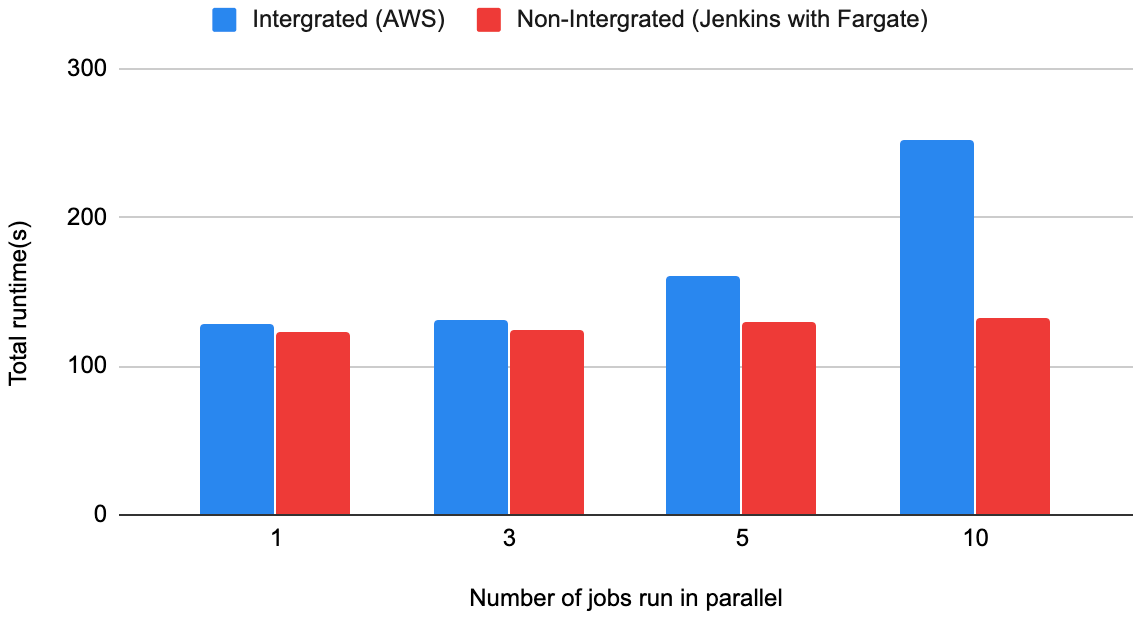
\includegraphics[width=0.80\textwidth]{pics/compare-aws.png}
  \caption{Runtime of the pipeline with on Different Toolchain}
  \label{fig:compareaws}
\end{figure}
Figure \ref{fig:compareaws} shows the result of this experiment. The runtime of integrated toolchain increases with the number of the task runs in parallel, while the non-integrated toolchain remains stable regardless of the number of parallel tasks. We will analyse the reason later in this section.
\par
From Figure \ref{fig:stage_runtime}, we can see that during the execution of a single job, tow toolchains have similar runtime. The similar runtime is because the build stage, which takes most of the runtime, is running in a similar environment in both toolchains. Both execution environment is within a Docker container runs with the same hardware in AWS. Although, the Docker image for the container is different in two toolchains, and we are not sure what if the actual hardware is the same since we have no visibility to the hardware in both toolchains. However, still, the performance is not so different in both toolchains.
\par
We further observe the time allocation between stages within the runtime in both toolchains. The figure shows our observation. To get the runtime in Figure \ref{fig:stage_runtime}, we run the pipeline in each toolchain for five times and get the average runtime of each stage. The first difference shows in Figure \ref{fig:stage_runtime} is that the Git Checkout stage in AWS integrated toolchain does not run on the container build agent. Instead, it is running in the unknown environment fully managed by AWS.
\begin{figure}[!h]
  \centering
  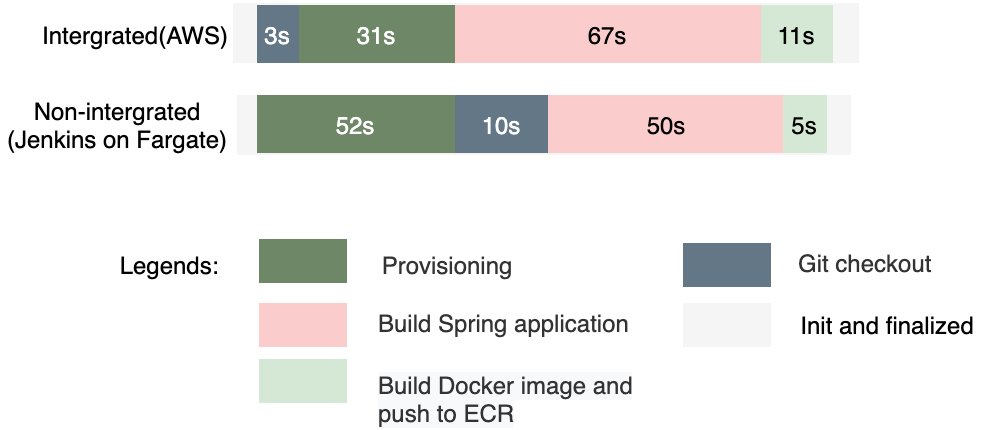
\includegraphics[width=0.99\textwidth]{pics/stages.png}
  \caption{Observation of Runtime of Each Stage on Two Toolchains}
  \label{fig:stage_runtime}
  \end{figure}
\par
We also compared used GitHub and use CodeCommit for the source control in the AWS integrated toolchain. 
We observed that it takes 10 seconds to do the git checkout when using third-party tools (GitHub) as the source control system. During these 10 seconds, the actual Git checkout only takes around 5 seconds, while the AWS toolchain does not do anything in the first 5 seconds. We presume that AWS provisions environment for runs the Git checkout stage in this 5 second, so this stage is also running in a serverless environment within AWS. However, we are not allowed to configure anything in this environment. In contract, it only takes 3 seconds to check out new code from CodeCommit and no waiting time before the checkout. This speed difference could because of the CodeCommit is the part of the AWS services. Thus it has faster data transfer between CodePipeline, or because of no environment provision needed before checkout.
\par
 The second difference is that in AWS integrated toolchain, the provisioning of the build environment is much faster. We presume this is due to AWS manages both build agent and this toolchain, and AWS is optimising the provisioning process of the build environment. Furthermore, the cloud instance that runs build environment in CodeBuild might already be started (used for the build task of other users) before CodePipeline sends our build job to CodeBuild. On the other hand, instances (Fargate) that run Jenkins agents is a cold start, which means it is not running before we send build job there.
 Nevertheless, we can also notice that the build time in the AWS integrated toolchain takes a longer time. It is hard for us to find the reason since the hardware configuration used by AWS is unknown except the size of RAM and the number of virtual CPU.
\par
 Also, we observe that with the workload goes up, the runtime of AWS integrated toolchain increases with it. We already answered why the runtime of the pipeline in our non-integrated toolchain with agent runs in AWS Fargate does not change over time in Section 5.1.3. To explain this, we also check the runtime of each stage when runs several jobs in parallel. We notice that when it has multiple jobs runs in parallel, essential if the parallel jobs' number goes over 5. AWS will start limiting the resource allocation, which limits the number of jobs that runs at the same time. As a result, part of our running jobs has to enter the "Queued" status before entering the "Provisioning" stage. In 10 jobs we run in parallel for the experiment, the time spent for queuing for resource various from 1 second (get resource allocated directly) to 130 seconds. Among these ten jobs, four jobs were put into the queue before resource are available to them. Figure \ref{fig:queued} shows the distribution of queued time among jobs. This validates the claim from AWS about parallel execution ability, which we mentioned in Section \ref{aws_parallel}. However, the parallel pipeline execution is not fully in parallel but with some limitations on available resources.
 \begin{figure}[!h]
  \centering
  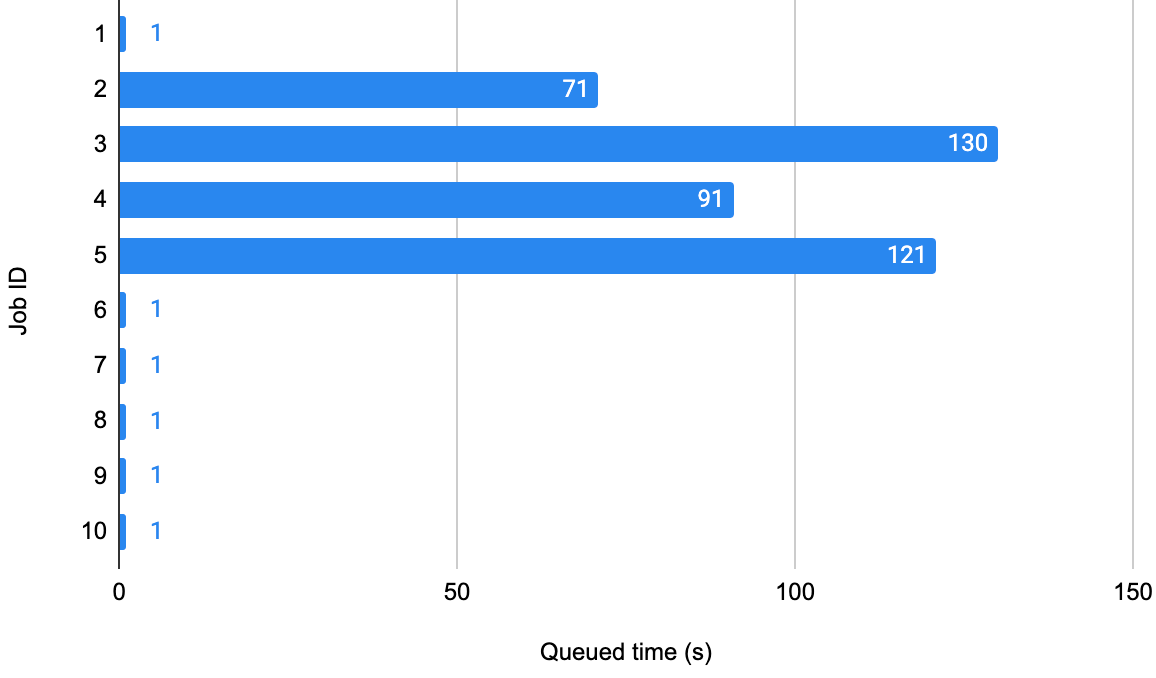
\includegraphics[width=0.90\textwidth]{pics/queued_time.png}
  \caption{Observation of Queued Time in AWS Integrated Toolchain During The runtime Experiment, When 10 Jobs Run in Parallel}
  \label{fig:queued}
\end{figure}
 \par
 The runtime of the non-integrated toolchain is also slightly going up because of the runtime of the build and push container to ECR increases. The reason is obvious, we have these two stages runs on the master node, so the increased data transfer between agent and master and limited computing resource on the Jenkins master increase the runtime. However, as we observed in Experiment 1, the build stage is always fully paralleled, and the runtime of this stage remains unchanged despite the increasing workload. The queuing time for resource in each job is negligible.
 \subsubsection{Cost Analysis}
 As a serverless tool, AWS DevOps tooling charges us according to the time and type of hardware configuration (in CodeBuild) we are using.
  Each pipeline in CodePipeline cost \$1 per month, which is a negligible amount of \$0.0014 per hour, price of with the build agent type general1.small (Linux instance with 3GB Memory and two vCPU) that we used in the experiment is \$0.3 per hour. The CodeDeploy is free of charge under the condition that we are not deploying to on-premises servers. The cost of S3 which store artifacts (<1 MB in our case) is negligible according to AWS\footnote{https://aws.amazon.com/getting-started/projects/set-up-ci-cd-pipeline/services-costs}. In conclusion, the price should be \$0.30014 per running job for one hour's runtime.
  \par
  In our non-integrated toolchain, our experiment setup (2 vCPU, 4 GB RAM) is different from what we have in 5.1. The price should be \$0.1029 per running agent for one hour's runtime. While the cost of EC2 instance that hosts the Jenkins master node costs \$0.0432 per hour, this price will remain constant when multiple jobs run in parallel. In general, the cost of the non-integrated toolchain is \$0.1452 per hour when only one agent is running.
From the calculation, we can see that the AWS integrated toolchain is more expensive under similar performance.
\subsection{Conclusion}
By analysing and explain the results, we could see that two toolchains have similar performance when it runs our case project. However, by further observe the runtime in each stage, we notice that the AWS integrated toolchain is faster in provisioning the build environment, but, slower in running the build and testing task itself. Such runtime distribution means it might be suitable for light but more frequent build task. 
The software project in real-life software development is much larger, and as a result, the build time will take a larger proportion in the total runtime. Therefore, the AWS integrated toolchain may become slower since it's building is slower than Jenkins non-integrated toolchain.
From the parallel execution part, we conclude that with our AWS integrated toolchain, the AWS CodeBuild, which takes most of the runtime, do have a limitation on the resource that we can use at the same time. Thus, before the system provisioning any resource, some tasks have to wait for the resource allocation in the "Queued" status. The "Queued" status largely prolongs the total runtime. 
\par
In general, the AWS integrated toolchain is more expensive and slower than our Jenkins-centred non-integrated toolchain, note that this does not mean the non-integrated is better than integrated toolchain. As we discussed in the last chapter, the AWS integrated toolchain is easier and faster to implement, is more stable and with better customer support. Table \ref{tab:exp2} summarised the result of this experiment.
\begin{table}[]
    \centering
    \begin{tabular}{|l|l|l|}
    \hline
     &
      \multicolumn{1}{c|}{\begin{tabular}[c]{@{}c@{}}Jenkins-centered \\ Non-integrated Toolchain\end{tabular}} &
      \multicolumn{1}{c|}{AWS Integrated Toolchain} \\ \hline
    Build Time &
      \begin{tabular}[c]{@{}l@{}}Slighter faster(123s), better \\ performance under parallel \\ build because Fargate \\ instances does not competing \\ for resources with each other.\end{tabular} &
      \begin{tabular}[c]{@{}l@{}}125s for a single task. \\ Increased with the number \\ of the parallel executing task \\ goes up, could be because \\ of the queueing for the\\ resources within CodeBuild.\end{tabular} \\ \hline
    Cost &
      \begin{tabular}[c]{@{}l@{}}Lower per hour price, \\ \$0.1452 per running \\ agent (includes the cost \\ of master node).\end{tabular} &
      \begin{tabular}[c]{@{}l@{}}Higher per hour price, \\ \$0.3 per hour per running \\ CodeBuild agent.\\ However no constant \\ additional cost as the master\\ node in Jenkins, might be \\ cheaper in a long run.\end{tabular} \\ \hline
    \end{tabular}
    \caption{Result of Experiment 2}
    \label{tab:exp2}
    \end{table}
% CONCLUSIONS AND FUTURE WORK
\chapter{Conclusions and Future Work}
\label{chp:conclusionsandfuturework}

\section{Conclusions}
TODO CONCLUSIONS

\section{Future Work}
TODO FUTURE WORK



% BIBLIOGRAPHY

\bibliographystyle{unsrt}
\bibliography{bib/article,bib/booklet,bib/inbook,bib/inproceedings,bib/misc,bib/phdthesis,bib/technicalreport,bib/book,bib/conference,bib/incollection,bib/manual,bib/mscthesis,bib/proceedings,bib/unpublished}
%\appendix

%\chapter{TODO APPENDIX NAME}
\label{app:}
Appendix body



\end{document}


